\documentclass[12pt, a4paper]{article}

\usepackage[utf8]{inputenc}
\usepackage[T1]{fontenc}
\usepackage[english]{babel}
\usepackage{geometry}
\geometry{margin=2.5cm}
\usepackage{needspace}
\usepackage{graphicx}
\graphicspath{{screenshot/}{plots/}{../screenshots/}}
\usepackage{amsmath}
\usepackage{amssymb}
\usepackage{listings}
\usepackage{xcolor}
\usepackage{hyperref}
\usepackage{booktabs}
\usepackage{caption}
\usepackage{subcaption}
\usepackage{float}
\usepackage{parskip}

% Code listing style
\definecolor{codebg}{RGB}{245,245,245}
\definecolor{codecomment}{RGB}{100,100,100}
\definecolor{codekeyword}{RGB}{0,0,180}
\definecolor{codestring}{RGB}{150,0,0}

\lstdefinestyle{cppstyle}{
    backgroundcolor=\color{codebg},
    commentstyle=\color{codecomment}\itshape,
    keywordstyle=\color{codekeyword}\bfseries,
    stringstyle=\color{codestring},
    basicstyle=\ttfamily\small,
    breakatwhitespace=false,
    breaklines=true,
    keepspaces=true,
    numbers=left,
    numbersep=8pt,
    numberstyle=\tiny\color{gray},
    showspaces=false,
    showstringspaces=false,
    tabsize=4,
    language=C++,
    frame=single,
    framesep=4pt,
    xleftmargin=12pt
}

\lstdefinestyle{glslstyle}{
    backgroundcolor=\color{codebg},
    commentstyle=\color{codecomment}\itshape,
    keywordstyle=\color{codekeyword}\bfseries,
    stringstyle=\color{codestring},
    basicstyle=\ttfamily\small,
    breaklines=true,
    numbers=left,
    numbersep=8pt,
    numberstyle=\tiny\color{gray},
    frame=single,
    framesep=4pt,
    xleftmargin=12pt,
    morekeywords={vec2, vec3, vec4, mat4, uniform, in, out, layout,
                  location, version, core, discard, normalize, dot,
                  sqrt, max, pow, texture, sampler2D}
}

\title{
    \textbf{GPU Ray-Casting of Quadric Surfaces} \\
    \large Implementation Report — Real-time Graphics Programming \\
    \large Università degli Studi di Milano
}
\author{Giorgia Carboni \and Betul Gul}
\date{Academic Year 2025--2026}

% -------------------------------------------------------------------------
\begin{document}
\maketitle
\tableofcontents
\newpage

% =========================================================================
\section{Introduction}
% =========================================================================

Molecular visualisation is a fundamental tool in structural biology and drug design. A common task is to display large protein molecules interactively, with correct shading and depth. Traditional polygon-based approaches (for example, rendering each atom as a sphere made of triangles) become slow when a molecule contains thousands of atoms, because the number of triangles grows quickly.

This report describes our incremental implementation of the method proposed by Sigg et al.~\cite{sigg2006}, \textit{GPU-Based Ray-Casting of Quadratic Surfaces}. The method represents atoms and bonds as mathematical surfaces (quadrics) and computes their appearance entirely on the GPU through ray-casting. This avoids the cost of polygon tessellation and produces pixel-perfect silhouettes and normals at any zoom level.

The project is written in C++17 using OpenGL~4.1, GLFW, GLAD, and GLM. It targets macOS compatibility (OpenGL 4.1 core profile). 

% =========================================================================
\section{Background}
% =========================================================================

\subsection{Quadric Surfaces}

A quadric surface is a second-degree algebraic surface. In homogeneous coordinates, it is defined by a $4 \times 4$ symmetric matrix $\mathbf{Q}$:
\begin{equation}
    \mathbf{p}^T \mathbf{Q} \, \mathbf{p} = 0
    \label{eq:quadric}
\end{equation}
where $\mathbf{p} = (x, y, z, 1)^T$ is a point on the surface. A sphere of radius $r$ centred at the origin corresponds to the diagonal matrix $\mathbf{Q} = \mathrm{diag}(1, 1, 1, -r^2)$.

\subsection{Ray-Quadric Intersection}

To find where a ray $\mathbf{r}(t) = \mathbf{o} + t\,\mathbf{d}$ hits the surface, we substitute into Equation~\ref{eq:quadric}:
\begin{equation}
    t^2 (\mathbf{d}^T \mathbf{Q} \mathbf{d})
    + 2t (\mathbf{o}^T \mathbf{Q} \mathbf{d})
    + \mathbf{o}^T \mathbf{Q} \mathbf{o} = 0
    \label{eq:rayquadric}
\end{equation}
This is a standard quadratic equation in $t$. If the discriminant is negative, the ray misses the surface.

In our implementation we solve Equation~\ref{eq:rayquadric} directly in eye space for spheres, rather than using the parameter-space transformation described in~\cite{sigg2006}. The parameter-space approach becomes numerically unstable under perspective at zoom-out, because the matrix inversion used in the transformation becomes ill-conditioned. Eye-space intersection avoids this problem and is mathematically equivalent for spheres.

\subsection{Impostor Technique}

Instead of sending one vertex per atom to the GPU, we generate a flat screen-facing quadrilateral (a \emph{billboard} or \emph{impostor}) around each atom centre. The fragment shader then performs the ray-sphere intersection for each pixel covered by the quad. Pixels that miss the sphere are discarded with \texttt{discard}; pixels that hit the sphere receive the correct colour and depth. This produces a geometrically exact sphere with no tessellation artefacts.

\subsection{Deferred Shading}

Deferred shading separates geometry processing from lighting. In the geometry pass, the fragment shader writes surface properties (colour, normal, depth) into a set of textures called the G-buffer. In the lighting pass, a fullscreen quad reads those textures and computes the final colour. With this structure, we ensure that complex lighting is calculated only once per screen pixel, regardless of how many objects overlap.
\clearpage
% =========================================================================
\section{Project Architecture}
% =========================================================================
\begin{figure}[h!]
    \centering
    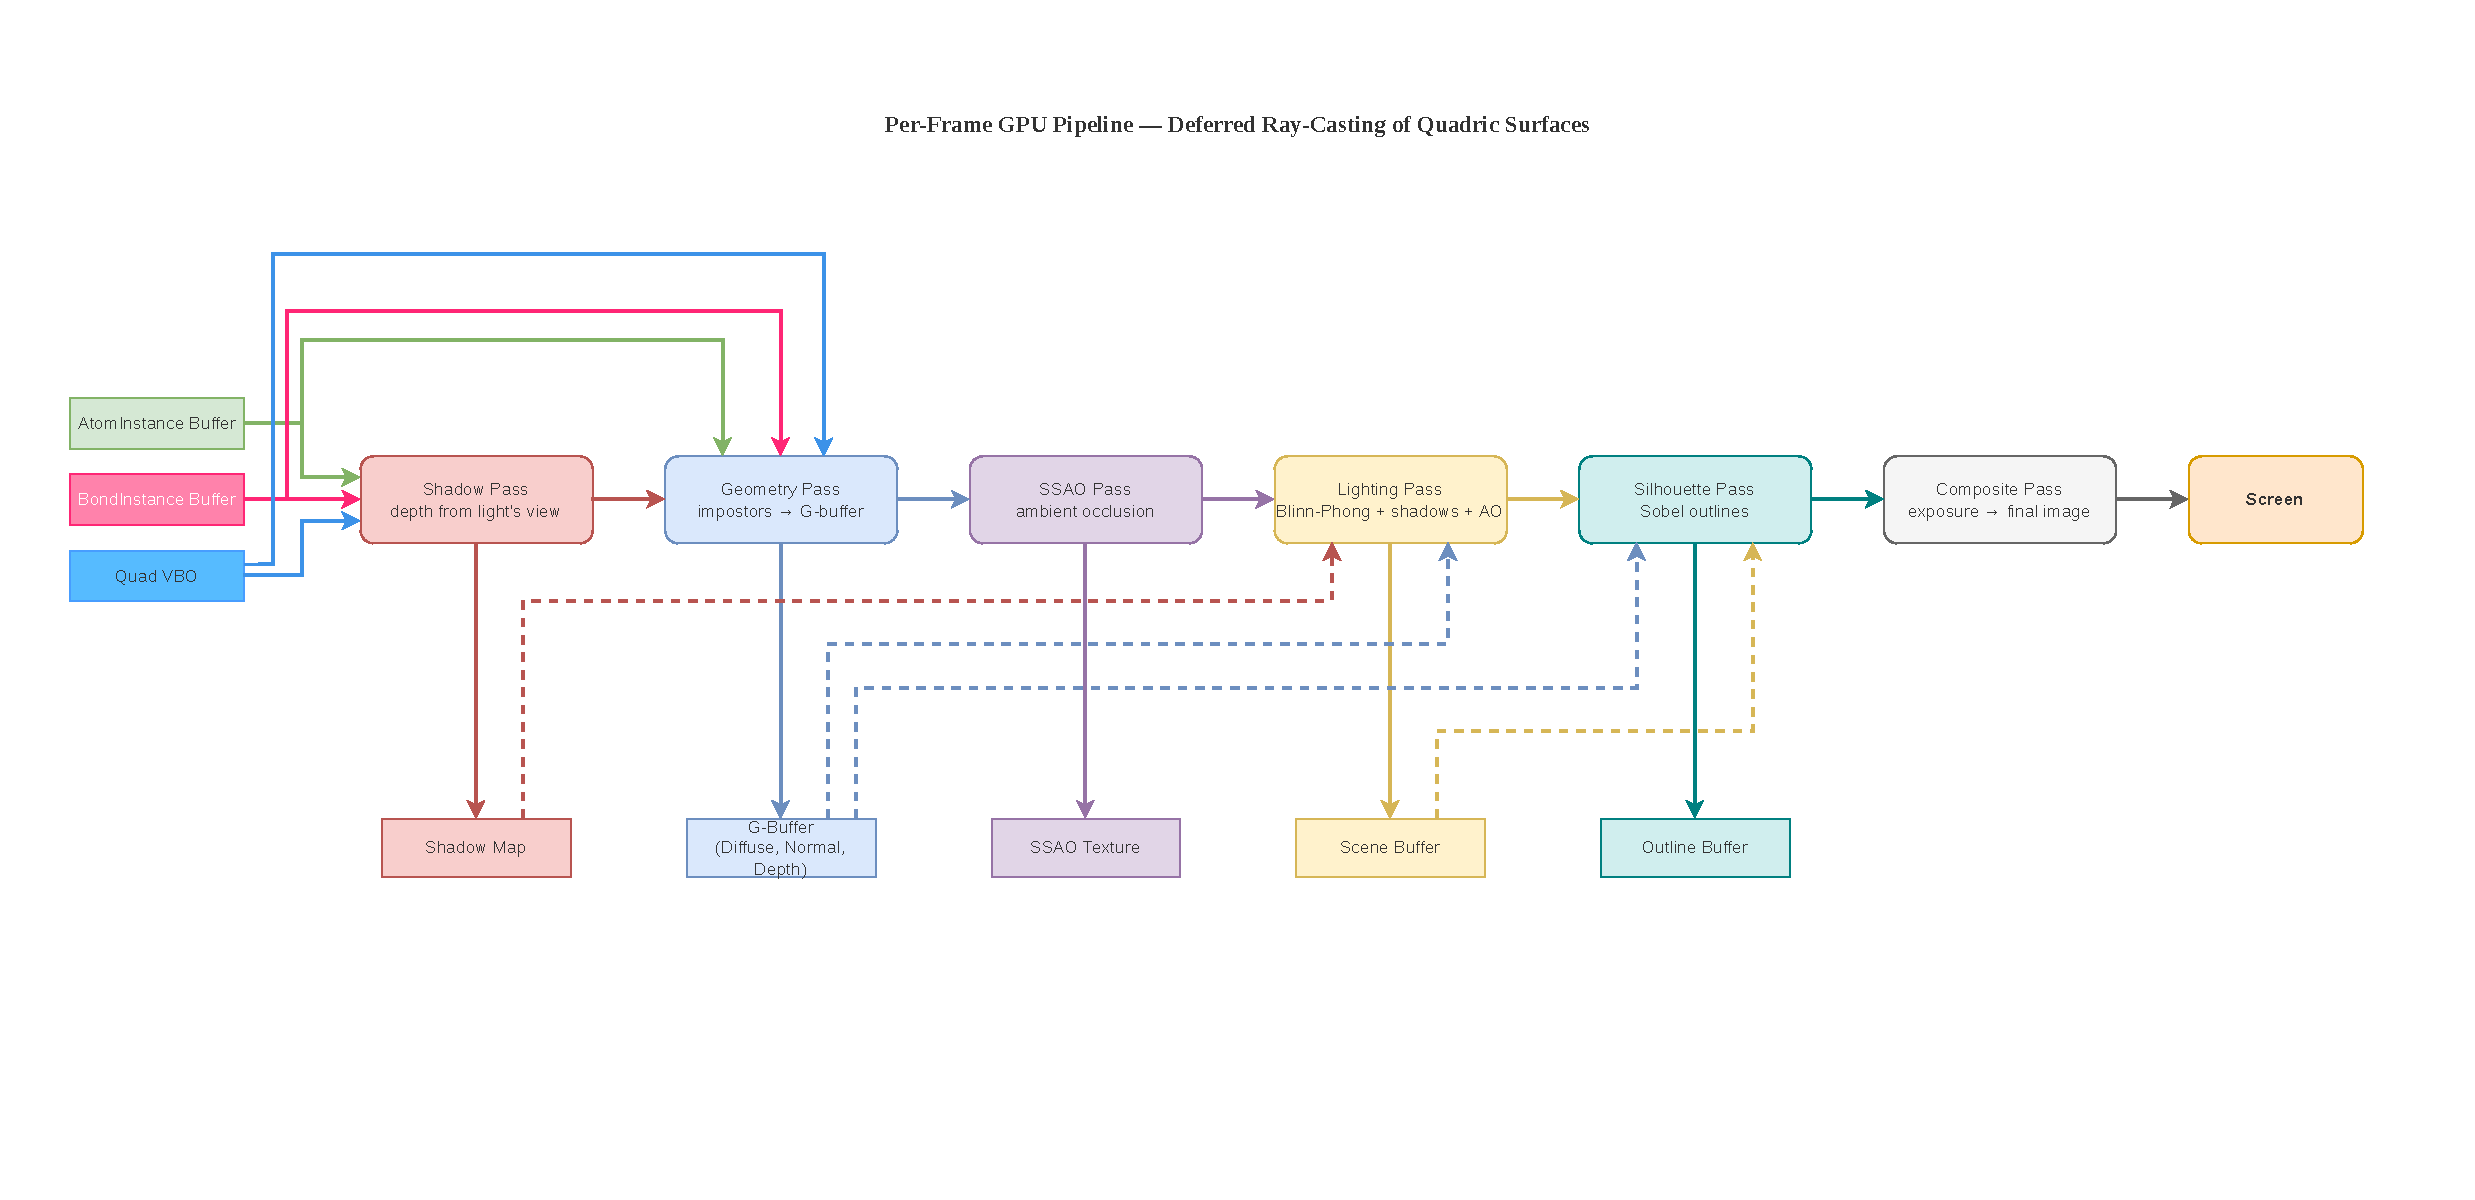
\includegraphics[width=\textwidth]{pipeline.pdf}
    \caption{Per-Frame GPU Pipeline for Deferred Ray-Casting of Quadric Surfaces.}
    \label{fig:pipeline}
\end{figure}

The pipeline adopts a \textbf{deferred shading architecture} so that the 
costly lighting, shadow, and ambient-occlusion computations execute 
exactly once per screen pixel, regardless of geometry overdraw. All 
sphere and cylinder impostors share a single \textbf{four-vertex quad VBO} 
rendered via instanced draw calls, with per-atom and per-bond data 
supplied through separate instance buffers; the vertex shader computes 
a \textbf{tight NDC bounding box} (Sigg et al., eq.~5) so each billboard covers 
only the pixels it actually contributes to. Ray--surface intersection 
is solved in \textbf{eye space} rather than the parameter-space transformation 
described in the paper, avoiding the numerical instability of matrix 
inversion under perspective at zoom-out. The six passes are described 
in detail in the sections that follow (Figure~\ref{fig:pipeline}).


% =========================================================================
\section{Implementation}
% =========================================================================

\subsection{Camera}

The \texttt{Camera} class implements an orbit camera parametrised by yaw angle $\phi$, pitch angle $\theta$, and distance $d$ from a target point. The camera position in world space is:
\begin{equation}
    \mathbf{pos} = \mathbf{target} + d \begin{pmatrix} \cos\theta \sin\phi \\ \sin\theta \\ \cos\theta \cos\phi \end{pmatrix}
\end{equation}
The view matrix is computed with \texttt{glm::lookAt}. The projection matrix uses \texttt{glm::perspective} with a $45^\circ$ vertical field of view, near plane $0.1$~\AA, and far plane $500$~\AA.

Mouse drag updates $\phi$ and $\theta$ (orbit); scroll updates $d$ (zoom). Pitch is clamped to $\pm 89^\circ$ to prevent the camera from flipping past the poles.

\subsection{Molecule Loading}

\subsubsection{PDB Parser}

The \texttt{PDB} class parses Protein Data Bank files~\cite{pdb}. Structures are downloaded from the RCSB Protein Data Bank (\url{https://www.rcsb.org}), which provides free public access to macromolecular structure data. The parser reads \texttt{ATOM} and \texttt{HETATM} records, extracting the $(x, y, z)$ coordinates and element symbol of each atom. After loading, all positions are translated so that the bounding box centre lies at the world-space origin.

The \texttt{getAtomStyle} method returns the CPK colour~\cite{cpk} and van der Waals radius~\cite{bondi1964} for each element. Table~\ref{tab:cpk} shows the values for the most common elements.

\begin{table}[H]
    \centering
    \begin{tabular}{llll}
        \toprule
        Element & CPK Colour (RGB) & vdW Radius (\AA) \\
        \midrule
        H  & White  (1.00, 1.00, 1.00) & 1.20 \\
        C  & Dark grey (0.35, 0.35, 0.38) & 1.70 \\
        N  & Blue  (0.19, 0.31, 0.97) & 1.55 \\
        O  & Red   (0.95, 0.15, 0.15) & 1.52 \\
        S  & Yellow (1.00, 0.78, 0.20) & 1.80 \\
        \bottomrule
    \end{tabular}
    \caption{CPK colours and van der Waals radii for selected elements.}
    \label{tab:cpk}
\end{table}

\subsection{Sphere Ray-Casting}

\subsubsection{Impostor Geometry}
To render the atoms efficiently, the system uses instanced rendering. This achieves the minimal data transmission model described in the paper, but implements it using modern hardware instancing.

The architecture is organized as follows: a compact \texttt{AtomInstance} record containing the center, radius, and CPK color is sent to the GPU for each atom. A standard quad template is then reused as the shared geometry for all the instances.

On the GPU side, the vertex buffer advances for each corner of the quad, while the instance buffer advances only once per atom via the \texttt{glVertexAttribDivisor} setting. As a result, thousands of atoms are rendered to the screen very fast through a single draw call:

\begin{lstlisting}[style=cppstyle]
glDrawArraysInstanced(GL_TRIANGLE_STRIP, 0, 4, static_cast<GLsizei>(atomInstances.size()));
\end{lstlisting}

This approach is critical for large molecules because it stores the atom data exactly once per instance, avoiding the need to duplicate the same data four times for the quad corners.

\subsubsection{Vertex Shader}

The vertex shader moves the atom centre to eye space, then expands each corner in the screen-aligned XY plane. Because XY in eye space corresponds to the screen plane, this keeps the quad always facing the camera. The NDC position of each corner is stored in the varying \texttt{vNDC} for use in the fragment shader.

\begin{lstlisting}[style=glslstyle, caption={billboard expansion in eye space (quadric.vert) }]
vec4 eyeCenter = uView * uModel * vec4(aCenter, 1.0);
vCenterEye = eyeCenter.xyz;

// Expand in eye-space XY 
eyeCenter.xy += aCorner * aRadius;
gl_Position = uProj * eyeCenter;

// Store NDC for ray reconstruction for avoiding framebuffer-size dependency
vNDC = gl_Position.xy / gl_Position.w;
\end{lstlisting}

The \texttt{vNDC} variable is preferred for ray reconstruction, as it eliminates the need to use \texttt{gl\_FragCoord} or \texttt{uViewport}. Since all four corners of the billboard geometry share the same clip-space $w$ value and the same eye-space $z$ depth, \texttt{vNDC} is linearly interpolated. This provides the exact NDC position at every fragment, independent of the framebuffer size. This is critically important for HiDPI Retina displays, where the framebuffer is larger than the window size.

\paragraph{Tight NDC bounding box (Sigg et al., eq.~5).}\label{sec:ndcbox}
To ensure the sphere is never clipped under perspective projection, we implement a tight NDC bounding box. Sigg et al.~\cite{sigg2006} provide a general implicit equation to find the screen-space boundaries ($b_x$) for any quadric:
$$(r_4^T D r_4)b_x^2 - 2(r_1^T D r_4)b_x + (r_1^T D r_1) = 0 \quad (5_{sigg})$$
While this matrix-based condition is universal, solving it on-the-fly for every vertex is computationally expensive. By analytically solving this tangency condition specifically for spherical geometry, we derive a direct formula for the billboard corners. For a sphere at eye-space position $(c_x, c_y, c_z)$ with radius $r$, let $Q_x = c_x^2 + c_z^2 - r^2$ and $f_x$ be the horizontal focal length. The NDC $x$-coordinate of each corner (with $s = \pm 1$ selecting left or right) is:

\begin{equation}
    x_{ndc} = -f_x \frac{c_x \sqrt{Q_x} - s r c_z}{c_z \sqrt{Q_x} + s r c_x} 
    \label{eq:spherenndc}
\end{equation}

The same formula applies for $y$ using $Q_y = c_y^2 + c_z^2 - r^2$ and $f_y$. This analytical derivation of the tight bounding box matters when an atom is close to the camera: a simple eye-space expansion underestimates the true screen extent and clips the sphere edges, while Equation~\ref{eq:spherenndc} ensures the quad always covers the sphere's silhouette exactly. When $Q \leq 0$, the camera is inside the sphere and the corner is set to cover the full screen edge. The depth component of \texttt{gl\_Position} is taken from the projected sphere centre, since the fragment shader overwrites \texttt{gl\_FragDepth} with the actual ray-sphere hit depth.

\subsubsection{Fragment Shader}

The fragment shader reconstructs an eye-space ray for each pixel from \texttt{vNDC} and the inverse projection matrix:

\begin{lstlisting}[style=glslstyle, caption={eye-space ray reconstruction and intersection (quadric.frag) }]
// Reconstruct eye-space ray
vec4 nearEye = uInvProj * vec4(vNDC, -1.0, 1.0);
vec4 farEye  = uInvProj * vec4(vNDC,  1.0, 1.0);
vec3 rO = nearEye.xyz / nearEye.w;  // ray origin (near plane)
vec3 rD = normalize(farEye.xyz / farEye.w - rO);  // ray direction

// Ray-sphere intersection (Eq. 2)
vec3  oc   = rO - vCenterEye;
float b    = dot(oc, rD);
float c    = dot(oc, oc) - vRadius * vRadius;
float disc = b * b - c;
if (disc < 0.0) discard;           // ray misses sphere
float t = -b - sqrt(disc);
if (t < 0.0) discard;              // sphere behind camera
\end{lstlisting}

If the ray hits the sphere, the fragment shader computes the hit position and surface normal in eye space, then writes the correct depth to \texttt{gl\_FragDepth}. This replaces the billboard depth with the true sphere surface depth, enabling correct occlusion between atoms.

\subsection{Deferred Shading}

\subsubsection{G-Buffer Setup}
The G-buffer is configured as an offscreen framebuffer with three distinct attachments. The first component, \textbf{Diffuse}, utilizes the \texttt{GL\_RGB8} format to store CPK colors obtained after diffuse shading. Since color values are naturally bounded within the $[0, 1]$ range, 8-bit precision is sufficient for this stage. In contrast, the \textbf{Normal} component is stored using the \texttt{GL\_RGB16F} format. This 16-bit floating-point precision is necessary because eye-space surface normals range between $[-1, 1]$, a signed interval that cannot be accurately represented in a standard \texttt{GL\_RGB8} buffer. To optimize storage, these normals are packed into the $[0, 1]$ range via the transformation $n' = n \times 0.5 + 0.5$ before being stored, and are subsequently unpacked during the lighting pass. Finally, per-pixel depth information written via \texttt{gl\_FragDepth} is stored in a \texttt{GL\_DEPTH\_COMPONENT24} attachment, effectively completing the decoupling of geometric data from lighting calculations.

\subsubsection{Geometry Pass}

In the geometry pass, the G-buffer FBO is bound before drawing. The sphere fragment shader writes to two colour attachments simultaneously using \texttt{glDrawBuffers}:

\begin{lstlisting}[style=glslstyle, caption={ G-buffer outputs (quadric.frag)}]
layout(location = 0) out vec4 oDiffuse;  // attachment 0
layout(location = 1) out vec4 oNormal;  // attachment 1

oDiffuse = vec4(vColor * diff, 1.0);
oNormal  = vec4(normalEye * 0.5 + 0.5, 1.0);
\end{lstlisting}

\subsubsection{Lighting Pass}

After the geometry pass, the default framebuffer is bound and a fullscreen quad is rendered. The lighting fragment shader reads the three G-buffer textures and applies Blinn-Phong shading:

\begin{equation}
    \mathbf{c} = k_a \mathbf{c}_d + \max(\mathbf{N} \cdot \mathbf{L}, 0)\,\mathbf{c}_d \cdot \mathbf{c}_l + \max(\mathbf{N} \cdot \mathbf{H}, 0)^s \, k_s \, \mathbf{c}_l
    \label{eq:phong}
\end{equation}

where $\mathbf{c}_d$ is the diffuse colour from the G-buffer, $\mathbf{c}_l$ is the light colour, $\mathbf{N}$ is the surface normal, $\mathbf{L}$ is the light direction, $\mathbf{H}$ is the halfway vector, $k_a$ is the ambient strength, $k_s$ is the specular strength, and $s$ is the shininess exponent. The eye-space fragment position is reconstructed from depth and the inverse projection matrix, which avoids storing a separate position texture in the G-buffer.

 Background pixels with a depth value of 1.0 are discarded, ensuring the background color remains visible.

Figure~\ref{fig:lightpass} shows the result after the deferred pipeline was first connected, with Blinn-Phong shading applied to the sphere impostors.

\begin{figure}[H]
    \centering
    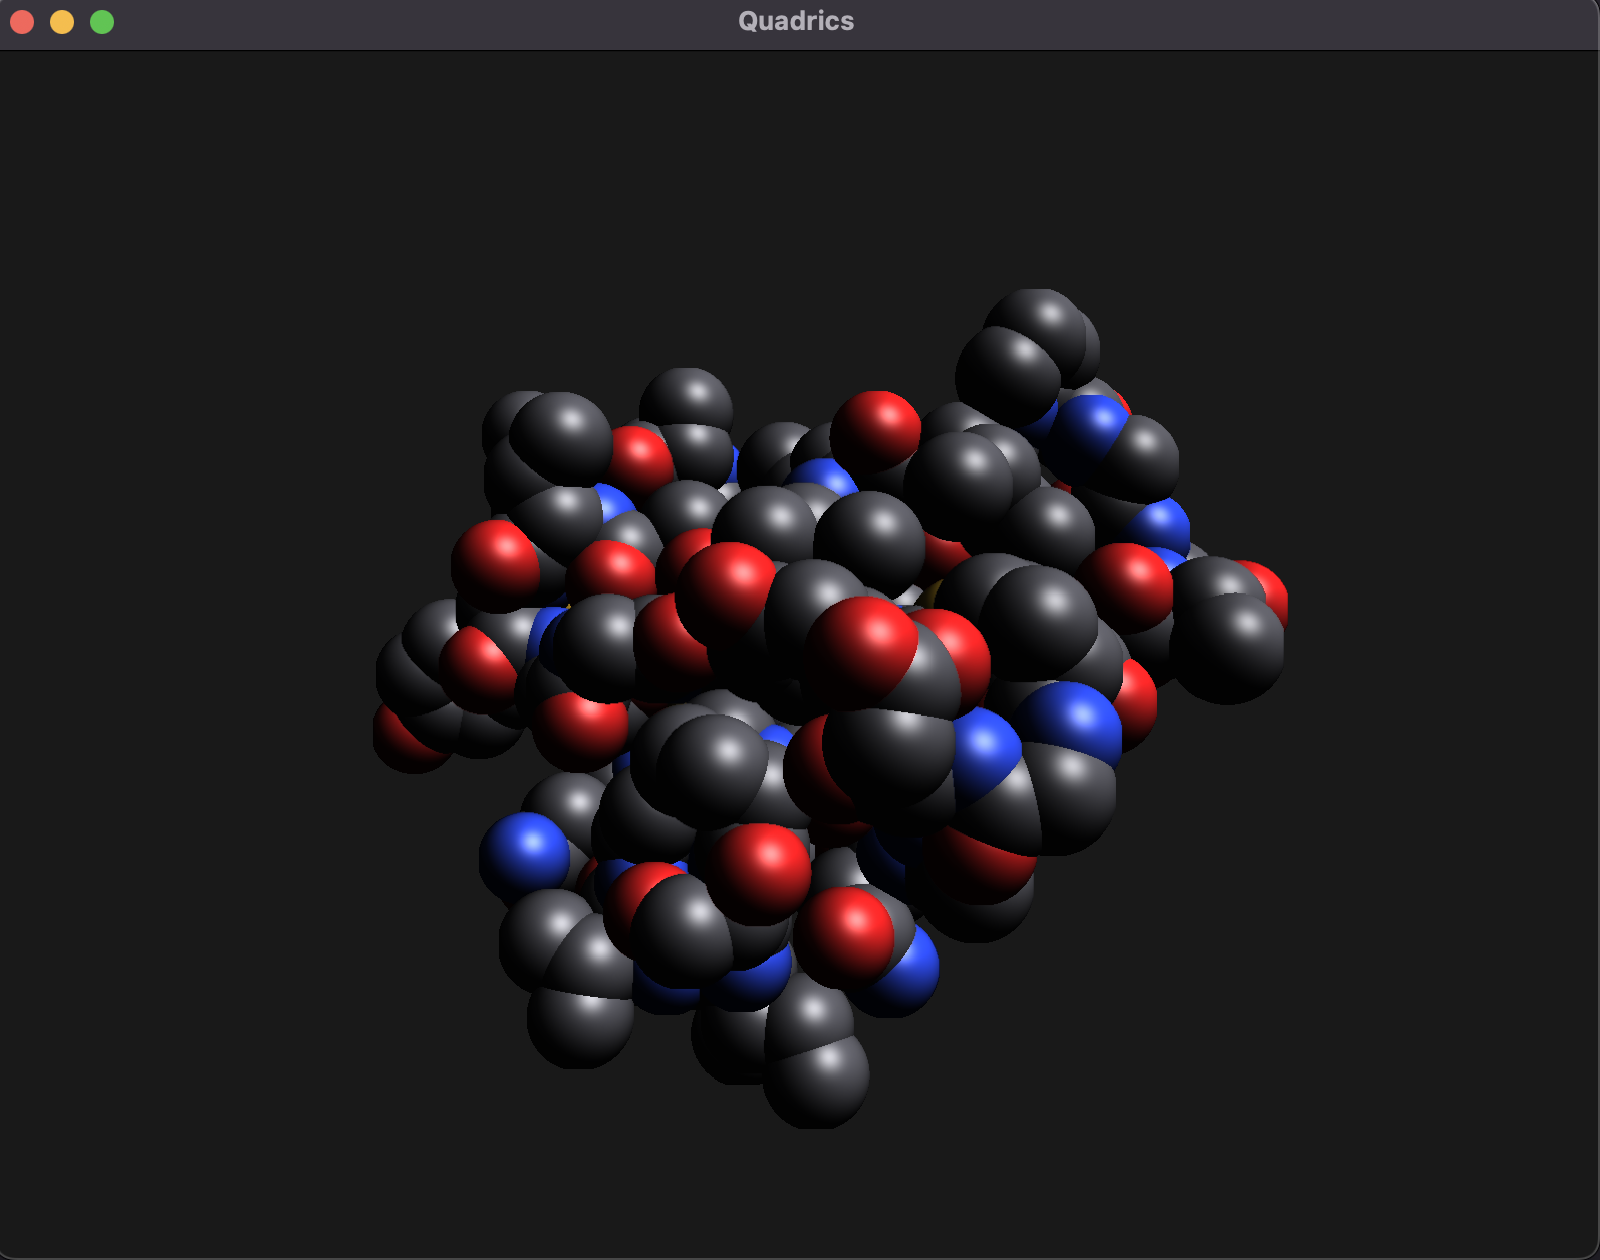
\includegraphics[width=0.7\textwidth]{quadric_first_light_pass.png}
    \caption{First successful deferred lighting pass: crambin (1CRN) with Blinn-Phong shading. The G-buffer stores diffuse colour, eye-space normal, and depth; the lighting pass reads all three and computes the final colour per pixel.}
    \label{fig:lightpass}
\end{figure}

\subsection{Bond Detection}

\subsubsection{Bonds Class}

The \texttt{Bonds} class detects covalent bonds by checking all atom pairs. Two atoms $A$ and $B$ are considered bonded if their distance satisfies:
\begin{equation}
    d(A, B) < r_{\mathrm{cov}}(A) + r_{\mathrm{cov}}(B) + \delta
    \label{eq:bond}
\end{equation}
where $r_{\mathrm{cov}}$ is the covalent radius of the element~\cite{alvarez2008} and $\delta = 0.45$~\AA\ is a tolerance that accounts for geometric variation.

\begin{lstlisting}[style=cppstyle, caption={Pairwise bond detection (Bonds.cpp)}]
for (size_t i = 0; i < atoms.size(); ++i) {
    for (size_t j = i + 1; j < atoms.size(); ++j) {
        float maxDist = getCovalentRadius(atoms[i].Element)
                      + getCovalentRadius(atoms[j].Element)
                      + tolerance;
        float dist = glm::length(atoms[i].Position - atoms[j].Position);
        if (dist < maxDist)
            List.push_back({i, j});
    }
}
\end{lstlisting}

Each bond is stored as a pair of indices into the atom array. This is an $O(N^2)$ algorithm, which is acceptable for proteins of a few thousand atoms. For molecule 1CRN (crambin, 327 atoms), the algorithm detects 337 bonds in negligible time.

\subsubsection{Cylinder Impostor Geometry}
\label{sec:cylcpu}

The cylinder GPU geometry follows the same instanced rendering design as spheres. Each bond becomes one \texttt{BondInstance} record uploaded once to the GPU:

\begin{lstlisting}[style=cppstyle, caption={BondInstance struct (one record per bond)}]
struct BondInstance {
    glm::vec3 PosA;   
    glm::vec3 PosB; 
    float     Radius; 
    glm::vec3 Color; 
};
\end{lstlisting}

The bond colour is the average of the CPK colours of the two bonded atoms. The cylinder radius is fixed at $0.15$~\AA\ for all bonds. The same shared 4-corner VBO used for spheres is reused here, keeping the draw call identical in structure:

\begin{lstlisting}[style=cppstyle]
glDrawArraysInstanced(GL_TRIANGLE_STRIP, 0, 4, numBonds);
\end{lstlisting}

\subsubsection{Cylinder Vertex Shader}

The cylinder vertex shader places the billboard corners at the exact screen-space boundary of the cylinder silhouette. Instead of a simple eye-space expansion, which clips cylinder edges at close range for the same reason described in Section~\ref{sec:ndcbox}, it applies the same Sigg et al. tangent-line formula (eq.~\ref{eq:spherenndc}) to both endpoints of the bond and takes the union of the two resulting boxes.

For a bond with eye-space endpoints $A$ and $B$, both treated as spheres of radius $r$, the billboard NDC $x$-edges are:
\begin{equation}
    x_{\mathrm{left}} = \min(x_1^A, x_2^A, x_1^B, x_2^B), \qquad x_{\mathrm{right}} = \max(x_1^A, x_2^A, x_1^B, x_2^B)
    \label{eq:cylndcbox}
\end{equation}
where $x_1$ and $x_2$ are the two tangent NDC values from (eq.~\ref{eq:spherenndc}) evaluated at that endpoint with $s = +1$ and $s = -1$ respectively. The same computation is applied for $y$. The corner selection then uses \texttt{aCorner.x} to pick the left or right edge and \texttt{aCorner.y} for top or bottom, exactly as for the sphere. The depth of \texttt{gl\_Position} is taken from the bond midpoint; the fragment shader overwrites \texttt{gl\_FragDepth} with the real hit depth.

This union always covers the full cylinder silhouette for the bond lengths and viewing distances that occur in molecule rendering.

\subsubsection{Cylinder Fragment Shader}

The fragment shader reconstructs an eye-space ray from \texttt{gl\_FragCoord} and the inverse projection matrix (the same method as the sphere shader, using the \texttt{uViewport} uniform set to the actual framebuffer size). It solves the ray-cylinder intersection by decomposing the ray into components parallel and perpendicular to the bond axis $\hat{d}$:
\needspace{10\baselineskip} % 10
\begin{lstlisting}[style=glslstyle, caption={Axis-decomposed ray-cylinder intersection (cylinder.frag)}]
vec3  d   = normalize(vPosBEye - vPosAEye);
vec3  Q   = rO - vPosAEye;
vec3  qc  = Q  - dot(Q,  d) * d;   // Q perpendicular to axis
vec3  rc  = rD - dot(rD, d) * d;   // rD perpendicular to axis

float a    = dot(rc, rc);
float b    = dot(qc, rc);
float c    = dot(qc, qc) - vRadius * vRadius;
float disc = b * b - a * c;
if (disc < 0.0 || a < 1e-6) discard;
\end{lstlisting}

After selecting the nearest positive intersection along the ray, two cap tests reject fragments that fall outside the finite cylinder length:

\begin{lstlisting}[style=glslstyle]
float proj = dot(hit - vPosAEye, d);
if (proj < 0.0 || proj > len) discard;
\end{lstlisting}

The surface normal is the vector from the cylinder axis to the hit point, divided by the radius. The hit depth is written to \texttt{gl\_FragDepth} and the diffuse colour and packed normal are written to the G-buffer, consistent with the sphere shader.

\subsection{Ground Plane and Shadow Maps}

\subsubsection{Ground Plane}

A flat quad is positioned at $y = -r_{\text{bound}} - 0.5$~\AA\ beneath the molecule's bounding sphere to serve as a ground plane. This geometry utilizes the standard G-buffer outputs, specifically the diffuse colour and the packed eye-space normal, ensuring that the lighting pass automatically calculates its shading without the requirement for additional code. By maintaining consistency with the G-buffer data generated by spheres and cylinders, the ground plane integrates seamlessly into the deferred shading pipeline.

\subsubsection{Shadow Maps}

A depth-only FBO at $2048\times2048$ resolution (\texttt{GL\_DEPTH\_COMPONENT24}) 
is rendered once per frame from the light's point of view using an orthographic 
projection fitted to the molecule's bounding radius. Since the scene consists 
of analytical impostors rather than tessellated geometry, dedicated shadow 
shaders clip each billboard to its correct silhouette: sphere billboards 
discard fragments outside the unit circle ($|\texttt{vCorner}|^2 > 1$), 
cylinder billboards apply a 2D capsule signed-distance function in 
light-space NDC, and the ground plane uses a standard depth-only pass.

In the lighting pass, the G-buffer depth is first unprojected to eye space 
via \texttt{uInvProj}, then transformed to world space via \texttt{uInvView}, 
and finally projected into light space via \texttt{uLightSpaceMatrix} for 
the shadow map lookup. The implementation follows the approach described 
by Sigg et al.:

\begin{quote}
\textit{``The small-scale molecule structures lead to highly complex shadow 
maps, thus requiring 64 shadow map samples to avoid visible noise inside 
the penumbra region. For better performance, the first 8 samples are used 
to adaptively determine whether the full 64 samples are required.''}
\end{quote}

The shadow map is configured with \texttt{GL\_LINEAR} filtering and 
\texttt{GL\_COMPARE\_REF\_TO\_TEXTURE} (\texttt{GL\_LEQUAL}), so declaring 
the GLSL uniform as \texttt{sampler2DShadow} makes every \texttt{texture()} 
call a hardware bilinear depth comparison returning a smooth value in 
$[0,\,1]$. Sample offsets follow a Vogel disk distribution --- successive 
positions rotated by the golden angle for an even, non-clumping circular 
spread. The first 8 samples are evaluated; if they all agree (fragment 
fully lit or fully shadowed) the remaining 56 lookups are skipped. 
Otherwise the full 64-sample kernel is processed and averaged. The result 
is a continuous soft penumbra with no banding, as shown in 
Figure~\ref{fig:shadowsfinal}.

\begin{figure}[H]
    \centering
    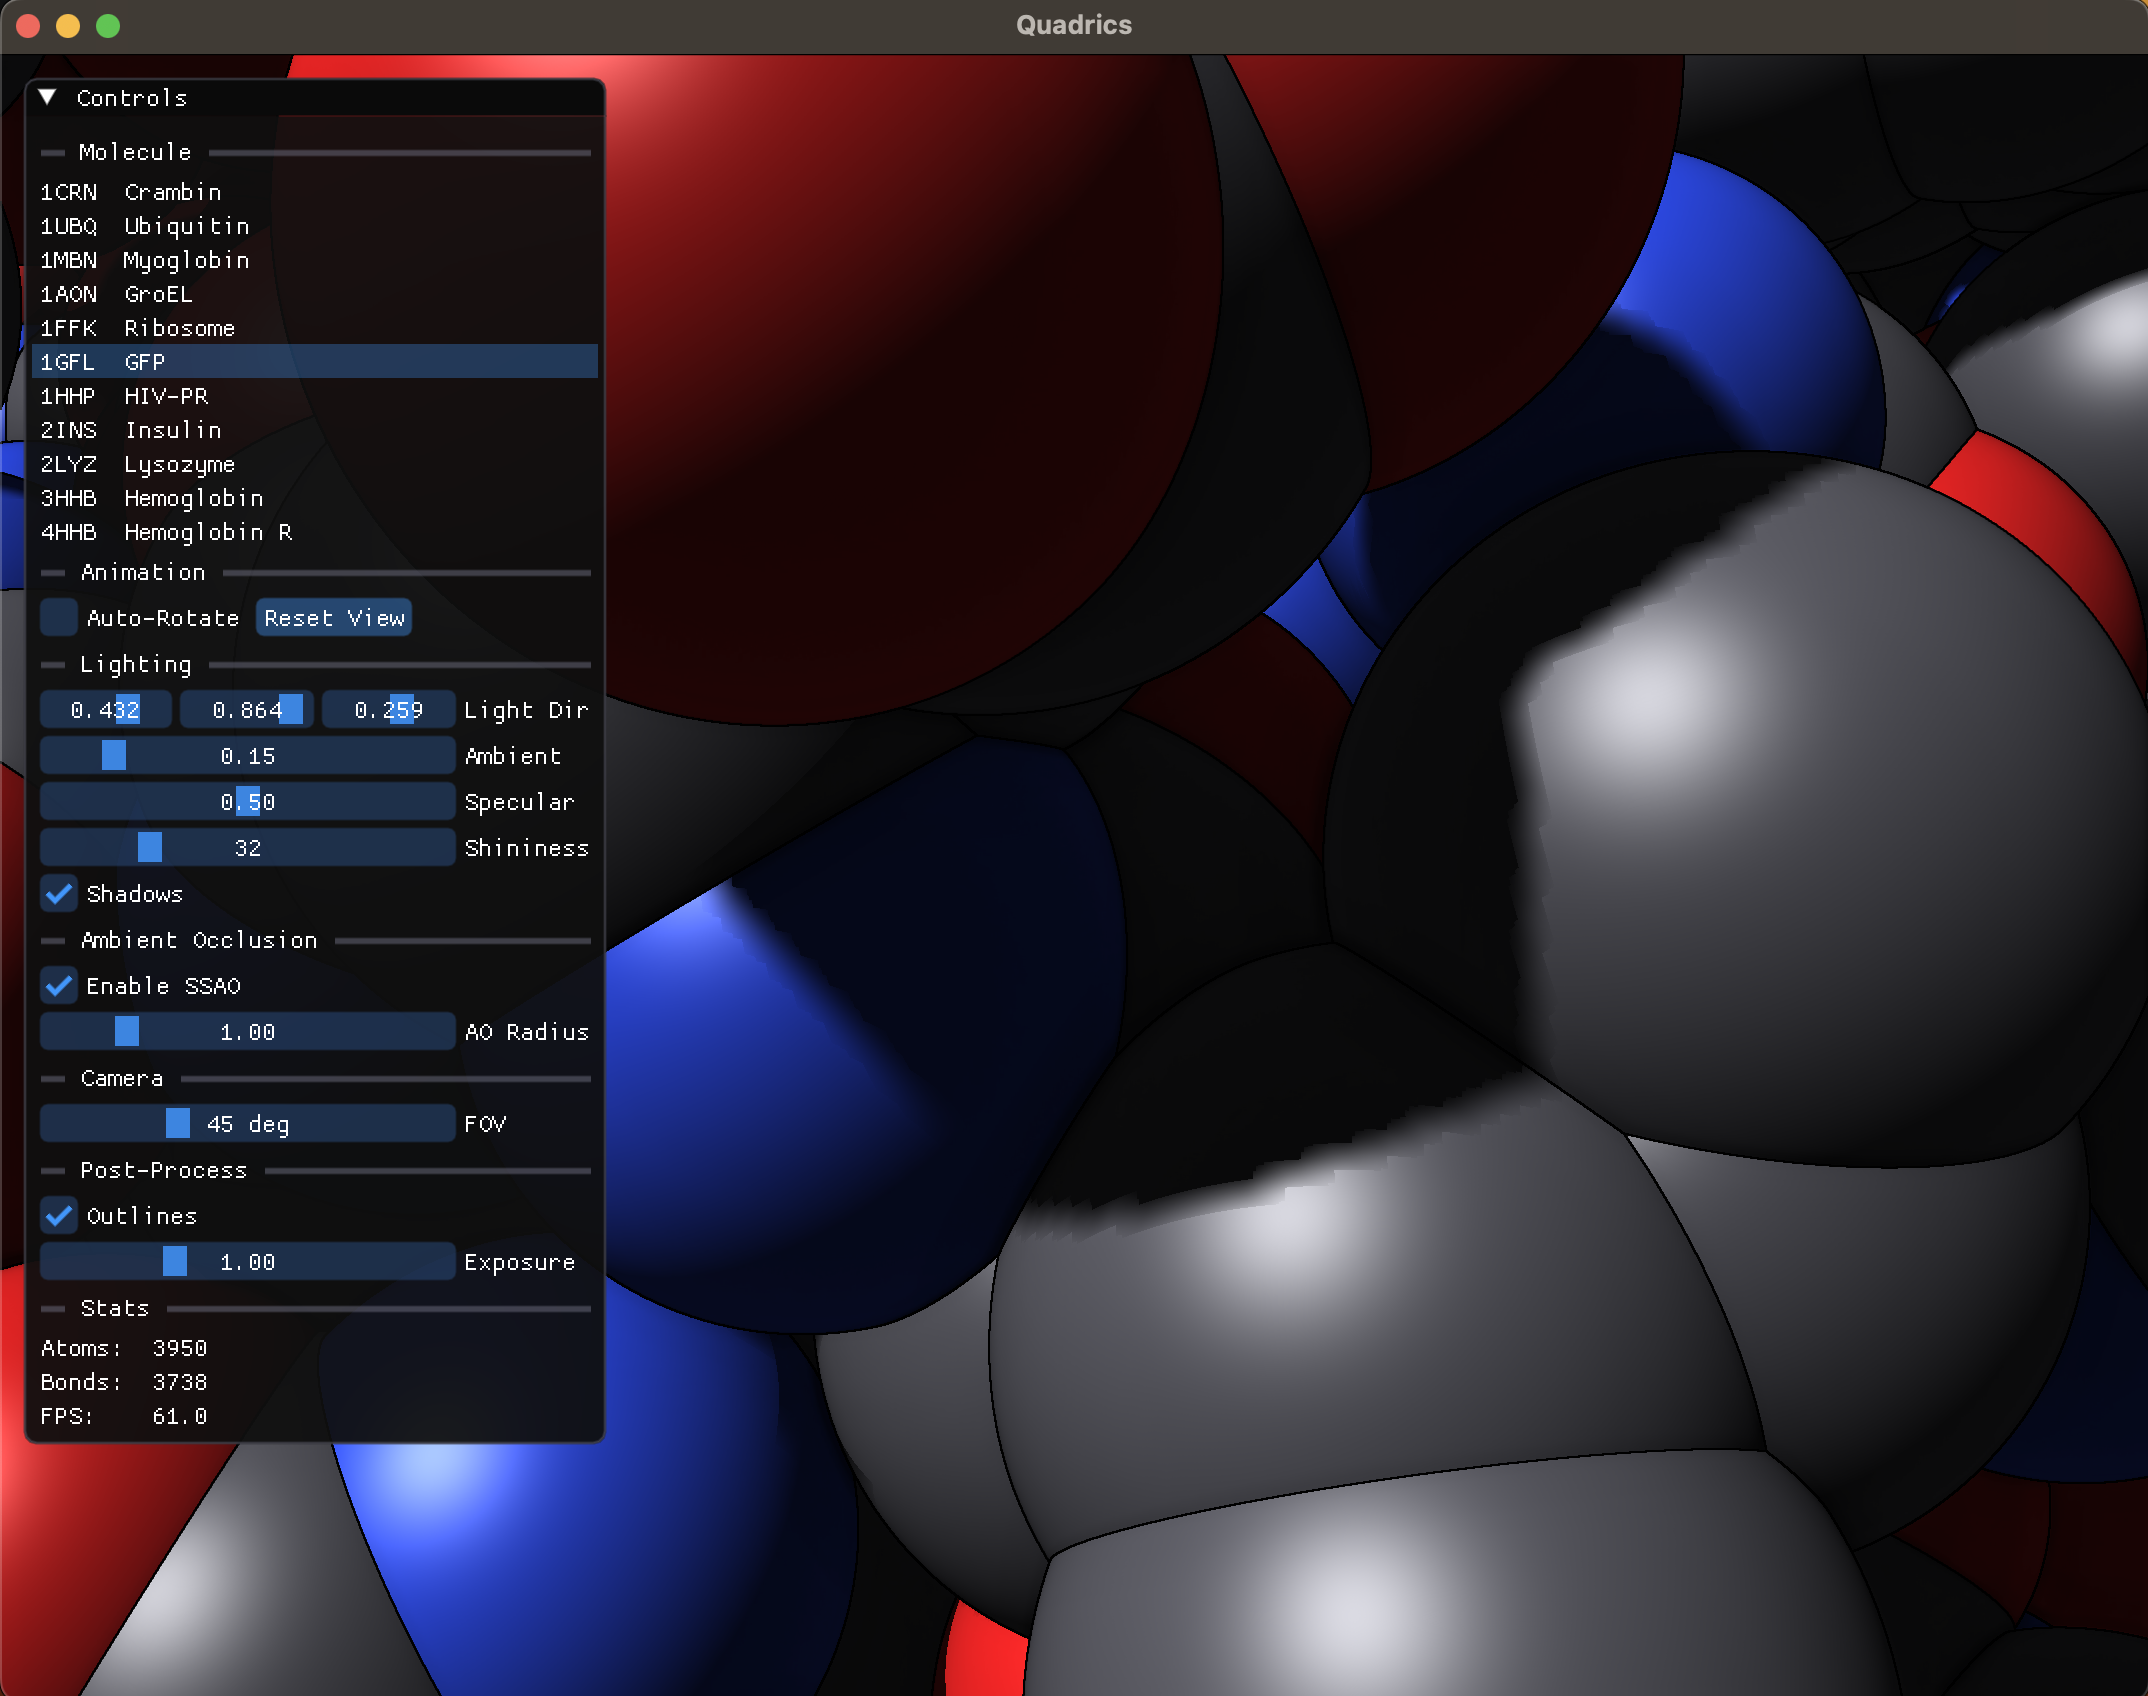
\includegraphics[width=0.70\textwidth]{shadows_final.png}
    \caption{Smooth penumbra produced by 64-sample adaptive hardware PCF 
    on the GFP molecule (1GFL). The soft falloff along the bottom-left 
    sphere is continuous, with no banding or stair-stepping. The 8-sample 
    early-out keeps the cost low: the frame rate stays above 60~fps.}
    \label{fig:shadowsfinal}
\end{figure}

\subsection{Screen-Space Ambient Occlusion}
\label{sec:ssao}

\subsubsection{SSAO Pass}

The SSAO pass reads the depth and normal textures from the existing G-buffer. For each fragment, 16 sample points are distributed in a hemisphere aligned with the surface normal. The hemisphere is rotated by a tiled $4\times4$ noise texture to break the regular banding pattern. Each sample is projected back into screen space and its depth compared against the G-buffer; samples that fall behind nearby geometry contribute to the occlusion value. A range-check weight (via \texttt{smoothstep}) avoids contributions from distant geometry. The result is written to a single-channel \texttt{GL\_R32F} texture, where $1.0$ means fully lit and $0.0$ fully occluded.

\subsubsection{SSAO Blur and Integration}

A second fullscreen pass applies a $4\times4$ box blur to remove the high-frequency noise from the small kernel. The blurred occlusion value is then multiplied into the ambient term in the lighting pass:
\begin{equation}
    \mathbf{c}_{\text{ambient}} = k_a \cdot \mathbf{c}_d \cdot \mathrm{ao}
    \label{eq:ssao}
\end{equation}
where $\mathrm{ao}$ is clamped to $[0.4,\,1.0]$ to prevent fully black contact areas. SSAO is applied exclusively to the ambient component of the lighting model, leaving the diffuse and specular terms unaffected.

% =========================================================================
\subsection{Post-Processing Refinement and System Interface}

\subsubsection{Silhouette and Crease Lines}
\label{sec:silhouette}

The paper proposes a non-photorealistic effect to make the molecule structure easier to read (Section 4, page 5):
\begin{quote}
\textit{``Silhouettes and creases can easily be detected by applying a Sobel edge detection filter to depth values and surface normals. The resulting gradient length can be considered as silhouette strength, which is finally used to blend the outline colour with the Phong lighting.''}
\end{quote}

We implemented this as a dedicated pass situated between the lighting and composite stages. This pass reads three textures: the lit scene from \texttt{sceneBuf}, alongside the depth and normal textures from the G-buffer. It then writes the lit scene, augmented with dark outlines, into a new \texttt{SceneBuffer outlineBuf}, which the composite pass subsequently reads instead of the original \texttt{sceneBuf}. Within this stage, the shader applies the Sobel operator twice to achieve precise edge detection. It is first applied to the depth buffer to detect silhouette edges, where depth values shift sharply between individual atoms or against the background. Simultaneously, the operator is applied to the normal map to identify crease lines, which occur where the surface normal changes abruptly even at similar depths, such as the contact points between two touching atoms.
\needspace{10\baselineskip} % 10
The two gradient magnitudes are scaled to a roughly $[0, 1]$ range, the stronger of the two is taken, and the lit colour is blended toward black by that amount:
\begin{lstlisting}[style=glslstyle, caption={Sobel edge detection on G-buffer (silhouette.frag)}]
float edgeDepth  = sobelDepth (TexCoord, texel) * 20.0;
float edgeNormal = sobelNormal(TexCoord, texel) * 1.5;
float edge = clamp(max(edgeDepth, edgeNormal), 0.0, 1.0);

vec3 sceneColor = texture(uScene, TexCoord).rgb;
FragColor = vec4(mix(sceneColor, vec3(0.0), edge), 1.0);
\end{lstlisting}

The two scale factors (20.0 for depth, 1.5 for the normal map) bring each gradient into a comparable range and can be tuned to adjust outline thickness. The paper reports that this pass adds about 8\% of the total frame time on their hardware (page 6); on modern GPUs the cost is essentially zero because it is a single texture read per pixel with no heavy computation.

The effect can be toggled at runtime through the new ``Outlines'' checkbox in the Post-Process section of the ImGui panel. Figure~\ref{fig:sobel} shows the difference between the lit-only output and the same view with silhouette and crease lines applied.

\begin{figure}[H]
    \centering
    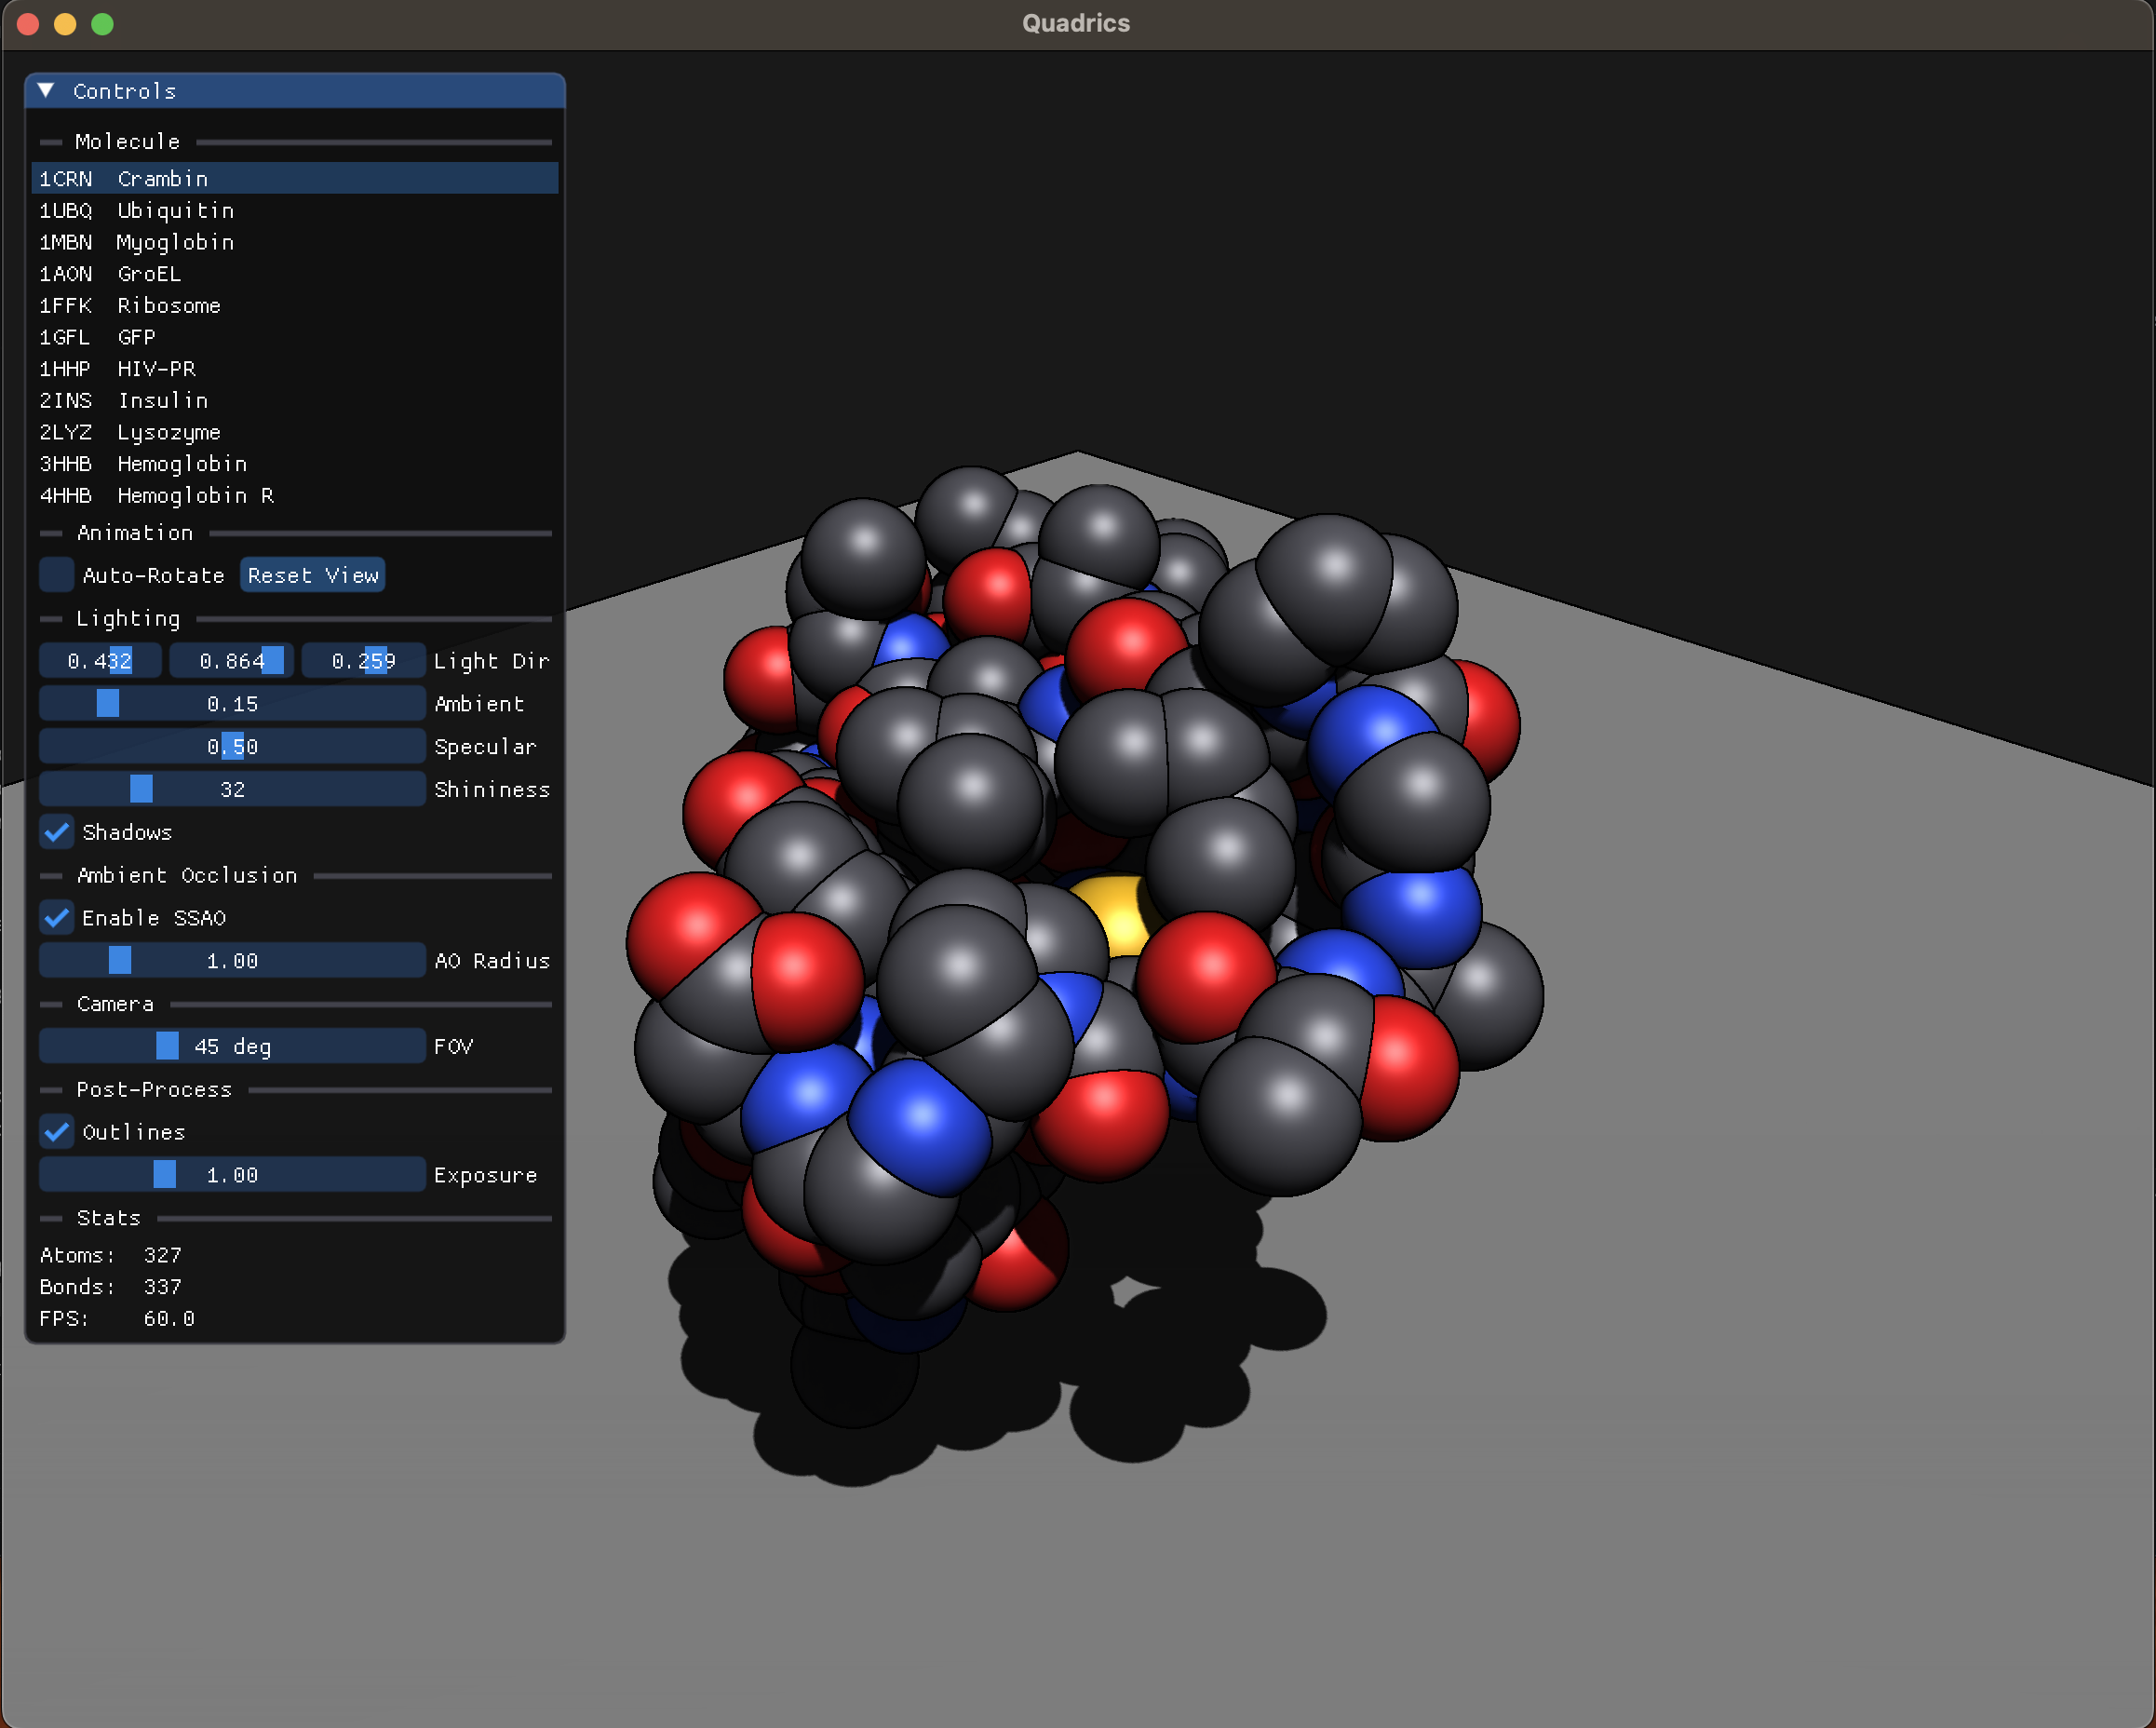
\includegraphics[width=0.85\textwidth]{sobel_contours.png}
    \caption{The full pipeline including Sobel silhouette and crease lines. The dark outlines emphasise atom boundaries (silhouettes) and the contact points between touching atoms (crease lines), greatly improving spatial perception of the molecular structure, exactly as described in Section 4 of Sigg et al.}
    \label{fig:sobel}
\end{figure}

\subsubsection{Composite Pass}

After the lighting pass, a dedicated composite pass applies image-wide adjustments before writing to the screen. The lighting pass now renders into an intermediate \texttt{SceneBuffer} (\texttt{GL\_RGB16F} FBO) instead of the default framebuffer. A fullscreen quad then samples that texture and multiplies by a uniform \texttt{uExposure}:

\begin{lstlisting}[style=glslstyle, caption={Exposure control (composite.frag)}]
FragColor = vec4(texture(uScene, TexCoord).rgb * uExposure, 1.0);
\end{lstlisting}

No tone mapping or gamma correction is applied. CPK atom colours are already chosen in perceptual (sRGB-like) space, so applying gamma would wash out the image rather than improve it. The intermediate buffer also provides a clean hook for future post-processing effects.

\subsubsection{ImGui Control Panel}

Dear ImGui is vendored into \texttt{external/imgui/} (core source files plus the GLFW and OpenGL3 backends). A floating panel is drawn on top of the composited image every frame, divided into labelled sections:

\begin{itemize}
    \item \textbf{Molecule} — selectable list of all 11 included PDB structures; switching triggers a runtime reload (VBOs are re-uploaded with \texttt{glBufferData}, the ground plane and camera are reset to fit the new molecule).
    \item \textbf{Animation} — auto-rotate toggle and a ``Reset View'' button that restores the initial camera pose.
    \item \textbf{Lighting} — light direction (three-axis slider), ambient strength, specular strength, shininess exponent, and a shadows on/off checkbox that bypasses the PCF lookup in the lighting pass.
    \item \textbf{Ambient Occlusion} — enable/disable SSAO checkbox; AO radius slider, shown only when SSAO is active.
    \item \textbf{Camera} — vertical field of view.
    \item \textbf{Post-Process} — outlines on/off checkbox (Section~\ref{sec:silhouette}) and exposure multiplier.
    \item \textbf{Stats} — live atom count, bond count, and frame rate.
\end{itemize}

Mouse and scroll callbacks check \texttt{ImGui::GetIO().WantCaptureMouse} before forwarding events to the camera, so dragging a slider does not also orbit the molecule. Figure~\ref{fig:imgui} shows the final control panel.


\begin{figure}[H]
    \centering
    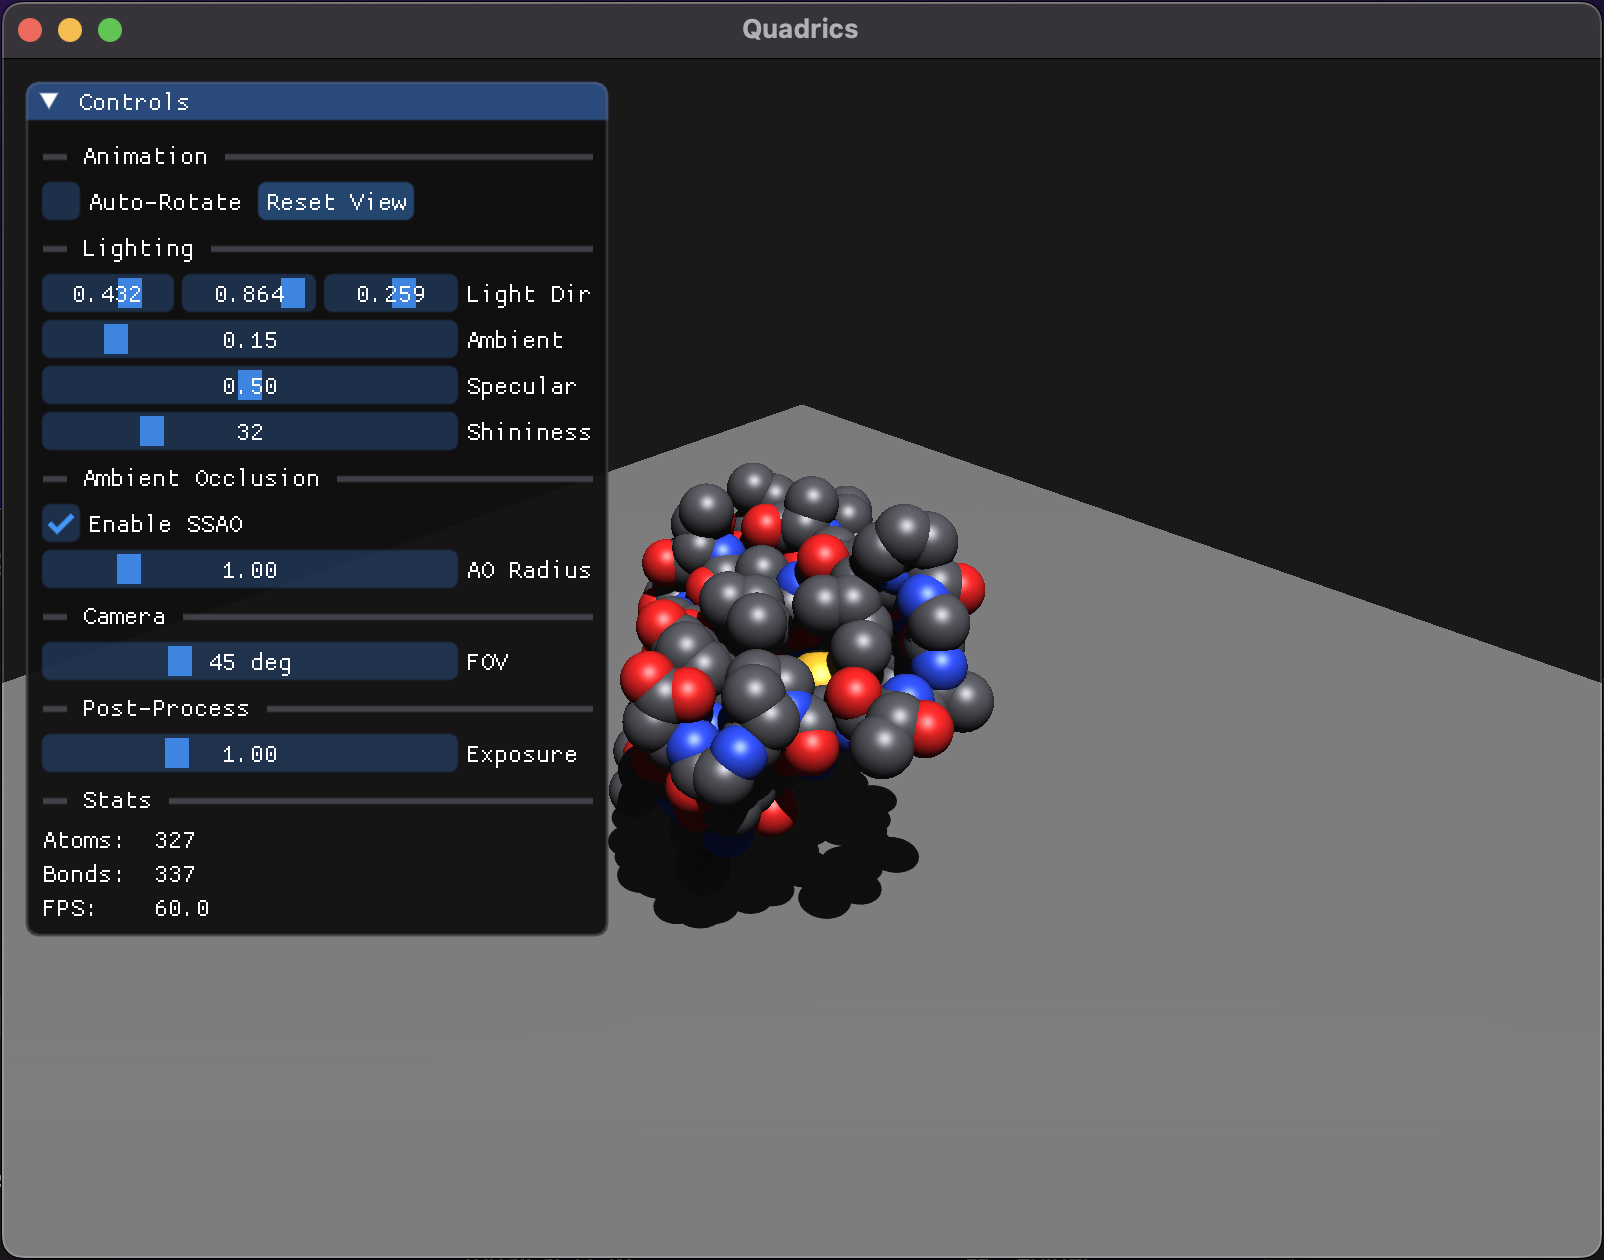
\includegraphics[width=0.70\textwidth]{first_imgui_menu.png}
    \caption{The ImGui control panel overlaid on the rendered scene. Molecule selection, lighting parameters, SSAO, camera FOV, and live stats are all adjustable at runtime without recompiling.}
    \label{fig:imgui}
\end{figure}


\begin{figure}[H]
    \centering
    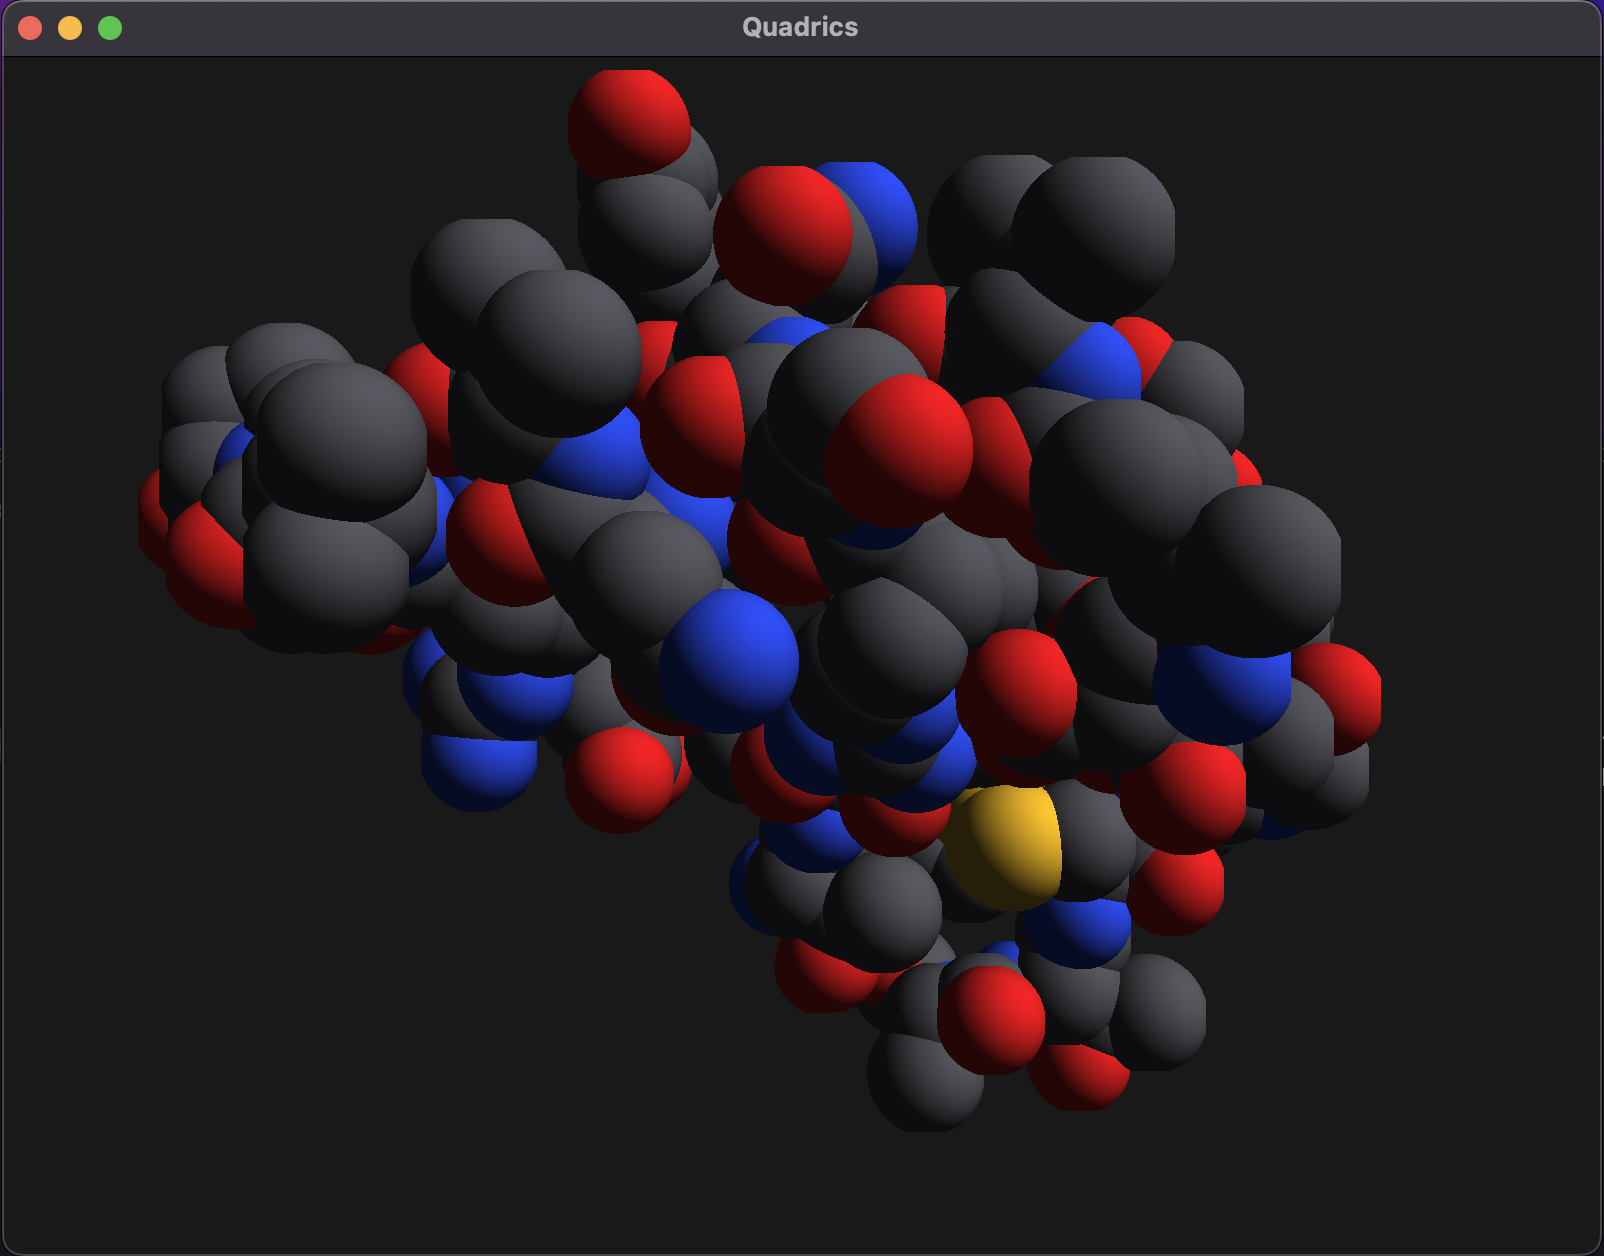
\includegraphics[width=0.48\textwidth]{first_quadric.png}
    \hfill
    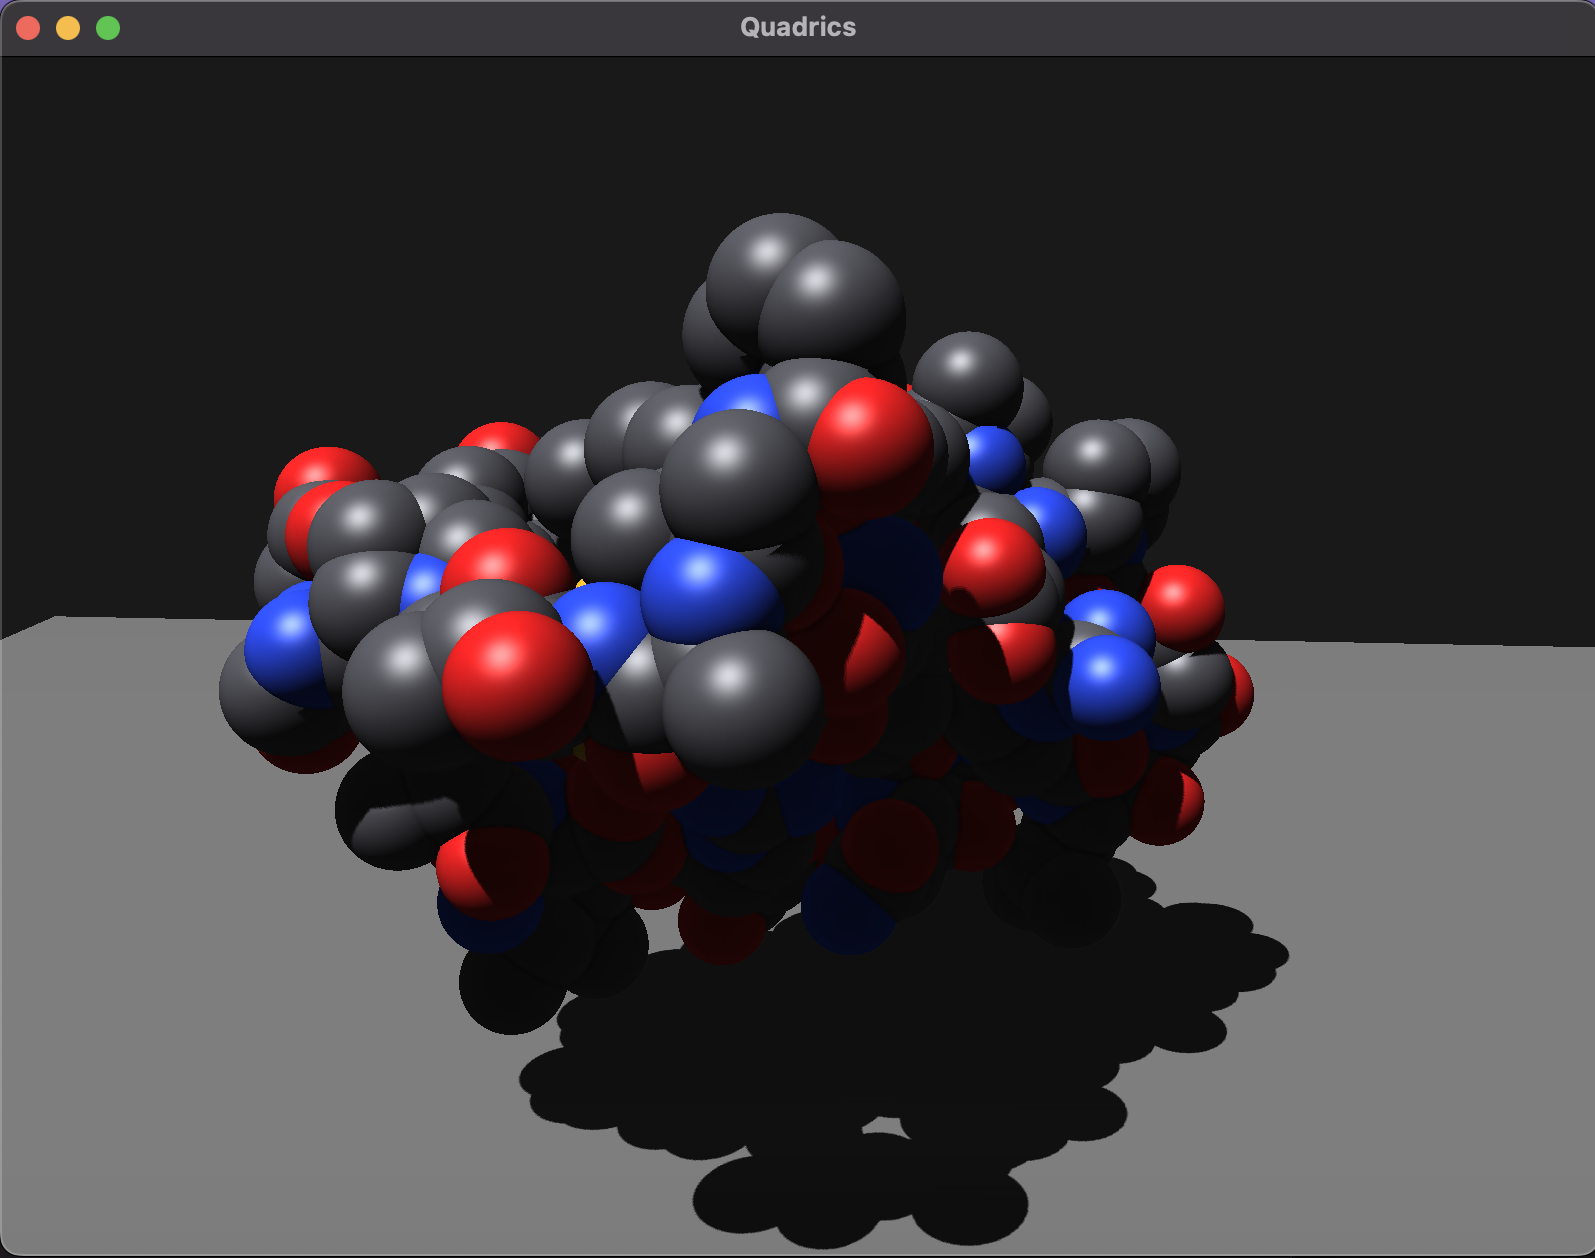
\includegraphics[width=0.48\textwidth]{quadric_light_and_shadows.png}
    \caption{Left: crambin (1CRN) after the initial deferred lighting pass (spheres only). Right: full pipeline — spheres, cylinders, ground plane, PCF shadows, and SSAO.}
    \label{fig:result}
\end{figure}

Figure~\ref{fig:result} shows the progression from the initial sphere-only lighting pass to the complete pipeline with cylinders, ground plane, shadows, and SSAO.

% =========================================================================
\section{Development Challenges}
% =========================================================================

\subsection{Resolution Scaling and High-DPI Display Adaptation}

On high-resolution environments such as macOS Retina displays, a significant discrepancy exists between logical window dimensions and physical framebuffer size, where the latter is typically twice the size of the former in each dimension. This scaling factor initially led to critical rendering artifacts, specifically regarding G-buffer allocation and ray reconstruction accuracy. 

The first technical challenge appeared when the G-buffer was initialized using static window constants such as \texttt{SCR\_WIDTH} and \texttt{SCR\_HEIGHT}. Since the actual framebuffer resolution was significantly higher (e.g., $1600 \times 1200$ for an $800 \times 600$ window), the resulting textures were insufficient for the physical pixel grid, causing the lighting pass to cover only the bottom-left quadrant of the screen. To resolve this, the pipeline was updated to utilize \texttt{glfwGetFramebufferSize} for all FBO allocations and viewport configurations, ensuring that resource dimensions always correspond to the physical pixel density:

\begin{lstlisting}[style=cppstyle]
glfwGetFramebufferSize(window, &fbWidth, &fbHeight);
gbuf.create(fbWidth, fbHeight);
\end{lstlisting}

A secondary challenge involved incorrect ray direction calculations within the fragment shader. Early iterations of the ray reconstruction logic relied on the ratio of \texttt{gl\_FragCoord.xy} to a \texttt{uViewport} uniform based on window size. On HiDPI systems, \texttt{gl\_FragCoord} operates in framebuffer pixel coordinates, leading to a normalized coordinate range of $[0, 2]$ instead of the expected $[0, 1]$, which invalidated the ray-marching logic. This dependency was eliminated by removing the viewport-based division and instead passing the Normalized Device Coordinate (NDC) position of each billboard corner as a varying from the vertex shader:

\begin{lstlisting}[style=glslstyle]
vNDC = gl_Position.xy / gl_Position.w;
\end{lstlisting}

Since all corners of a billboard share a consistent clip-space $w$ component, the \texttt{vNDC} value interpolates accurately across the fragment, allowing the shader to reconstruct rays independently of the underlying framebuffer resolution. This adaptation underscores a critical architectural lesson: on HiDPI systems, window and framebuffer dimensions must be treated as distinct quantities, and every resource matching the pixel grid must be explicitly sized using hardware-backed metrics.
% -------------------------------------------------------------------------
\subsection{G-Buffer Precision and Signed Data Normalization}

After connecting the deferred lighting pass, the shading started to look incorrect; some spheres were flat or very dark, independent of the light direction. The root cause of this was that the normal G-buffer texture was initially allocated with the internal format \texttt{GL\_RGB8}, which stores unsigned normalized values in the $[0, 1]$ range. Eye-space surface normals have components in the $[-1, 1]$ range. Although we packed the normal with $\text{normal} \times 0.5 + 0.5$ before storing it, because \texttt{GL\_RGB8} is an unsigned format, the GPU clamped the stored values to the $[0, 1]$ range before writing, and negative normal components were silently lost. To solve this problem, the normal attachment was changed to \texttt{GL\_RGB16F}, a 16-bit signed floating-point format that can represent the full $[-1, 1]$ range without clamping:

\begin{lstlisting}[style=cppstyle]
// Normals: 16-bit float, required for signed values in [-1, 1]
glTexImage2D(GL_TEXTURE_2D, 0, GL_RGB16F,
             w, h, 0, GL_RGB, GL_FLOAT, nullptr);
\end{lstlisting}

From this we understand that \texttt{GL\_RGB8} is an unsigned normalized format. Any G-buffer attachment that needs to store signed data, such as normals or motion vectors, requires a signed or floating-point format like \texttt{GL\_RGB16F} or \texttt{GL\_RGB16\_SNORM}.

\subsection{Dynamic Framebuffer Resizing}
Resizing the application window broke the rendering, causing the atoms to appear deformed and the image to be incorrectly scaled. Because all FBOs, such as the SSAO and scene buffer, were being allocated only at application startup to match the initial dimensions of the framebuffer. The \texttt{framebuffer\_size\_callback} function updated the \texttt{fbWidth}/\texttt{fbHeight} values and reset the viewport, but it never recreated the FBOs. On the next frame, because the geometry pass was writing to a texture with the old dimensions while the viewport expected the new dimensions, a corrupted output emerged. To fix this, we set a boolean flag named \texttt{fbDirty} to \texttt{true} in the resize callback. At the beginning of each render loop iteration, if \texttt{fbDirty} is set, we arranged it so that all four FBOs are destroyed and recreated at the current size before any rendering begins:

\begin{lstlisting}[style=cppstyle]
if (fbDirty && fbWidth > 0 && fbHeight > 0) {
    gbuf.create(fbWidth, fbHeight);
    ssaoBuf.create(fbWidth, fbHeight);
    ssaoBlurBuf.create(fbWidth, fbHeight);
    sceneBuf.create(fbWidth, fbHeight);
    outlineBuf.create(fbWidth, fbHeight);
    fbDirty = false;
}
\end{lstlisting}

This situation demonstrates that any FBO or texture that needs to match the screen resolution must definitely be recreated on every window resize, not only at startup.
% =========================================================================
\section{Anti-Aliasing in Deferred Rendering}
% =========================================================================

Edge quality is a known weak point of deferred rendering. Classical approaches like \textbf{Multi-Sample Anti-Aliasing (MSAA)} render each pixel at several sub-pixel positions and average the result. While this is efficient in forward rendering where shading occurs per sample directly on the geometry, deferred shading decouples geometry from lighting. Consequently, applying MSAA requires the G-buffer to store \emph{every sample} of diffuse colour, normal, and depth before the lighting pass executes. A $4\times$ MSAA setup therefore multiplies both memory bandwidth and lighting computation by four, defeating the primary architectural advantage of deferred shading. For this reason, MSAA is excluded from both our pipeline and the original paper's method.

The remainder of this section details how our ray-casting impostors mathematically mitigate most of the aliasing problem without relying on MSAA, outlining which residual artifacts were actively resolved (shadows) and which were deliberately retained (geometric silhouettes).

\subsection{Ray-Casting Mitigates the Problem Mathematically}

The aliasing that MSAA was designed to eliminate originates from tessellated polygons, where a sphere approximated by triangles produces straight edges that create visible staircases when crossing the pixel grid. Our impostors avoid this problem entirely. Each sphere and cylinder silhouette is computed by solving a quadratic equation per fragment (Section~\ref{sec:ndcbox}), so the edge of every primitive is mathematically defined, not approximated. The silhouette follows the smooth curve of the surface at fragment precision, not at polygon-edge precision.

What remains is a single residual: the \texttt{discard} at the impostor boundary is still a binary per-pixel decision, so the outermost row of pixels along a silhouette is either fully inside or fully outside. This produces a one-pixel-wide staircase. Compared to polygon meshes the artefact is barely visible because the staircase follows the smooth curvature of the sphere rather than the straight edges of triangles.

\subsection{Why We Did Not Add FXAA or SSAA}

\textbf{FXAA} is a post-process spatial filter that detects high-contrast edges in the final image and blurs them. It is compatible with deferred rendering (it runs after composite) and is cheap. However, FXAA cannot distinguish between a \emph{good} analytically computed edge and a \emph{bad} polygon edge: it would blur our mathematically correct silhouettes equally, degrading work that the fragment shaders just spent GPU cycles computing. The cure would be worse than the disease.

\textbf{SSAA} (Super-Sample Anti-Aliasing) renders the G-buffer at higher resolution and downsamples at composite. It is the correct solution for analytically defined surfaces because it preserves the mathematical silhouette. The cost, however, is prohibitive in our pipeline: a $1.5\times$ G-buffer roughly doubles the SSAO fill cost, and SSAO is already the most expensive pass. For molecules of a few thousand atoms the frame rate would drop below interactive.

\textbf{TAA} (Temporal Anti-Aliasing) is the modern industry standard but requires motion vectors, jittered camera offsets, and a history buffer. The implementation cost is much higher than the scope of this project.

\subsection{Perceptual Edge Enhancement via Sobel Filtering}

The paper does not implement geometric anti-aliasing at all. Instead, Sigg et al.\ improve \emph{perceptual} edge quality through a non-photorealistic effect: a Sobel edge detection filter applied to the G-buffer depth and normal textures. The resulting values are then blended as dark outlines on top of the Phong lighting as described in Section 4 on page 5. This approach addresses the perceptual challenge of distinguishing individual atoms from one another without introducing any pixel blurring. We have implemented this exact methodology, the details of which are provided in Section~\ref{sec:silhouette} and illustrated in Figure~\ref{fig:sobel}.

\subsection{Resolution of Shadow Penumbra Aliasing}

The geometric aliasing on silhouettes is subtle. The aliasing inside the soft shadow penumbra, however, was clearly visible in our earlier implementation. With \texttt{GL\_NEAREST} filtering and a 16-sample binary PCF, the soft shadow could only take 17 discrete values, producing a stair-stepped band along the penumbra edge. Two changes together remove this.

The first is hardware PCF: switching the shadow texture to \texttt{GL\_LINEAR} with \texttt{GL\_COMPARE\_\allowbreak{}REF\_TO\_\allowbreak{}TEXTURE} and declaring the GLSL uniform as \texttt{sampler2DShadow} makes every depth lookup a bilinear comparison, returning a smooth float in $[0, 1]$ rather than a binary $0$ or $1$. The second is a 64-sample adaptive PCF: increasing the kernel from 16 to 64 well-distributed Vogel-disk samples removes the remaining noise on complex molecule shadow maps, exactly as the paper prescribes (Section 4, page 5). The 8-sample early-out keeps the frame cost low, as most pixels still cost only 8 lookups.

Figure~\ref{fig:shadowsfinal} shows the result: the soft falloff along the shadow penumbra is now continuous, with no banding visible even at heavy zoom.
\subsection{Summary}

Our approach to edge quality in deferred rendering is therefore the combination of three deliberate choices: \textbf{ray-casting impostors} that give analytically correct silhouettes (so no MSAA/FXAA/SSAA needed for geometry); a \textbf{Sobel silhouette-and-crease pass} that handles the perceptual problem the paper highlights; and \textbf{64-sample adaptive hardware PCF} that removes the genuine aliasing inside the soft shadow penumbra. The result is a deferred pipeline that, despite the architectural absence of MSAA, produces clean edges throughout the image.

% =========================================================================
\section{Testing and Results}
% =========================================================================

\subsection{Hardware}

The two test machines represent two distinct GPU architectures.

\begin{itemize}
    \item \textbf{MacBook Pro 16,1 (2019)} --- 6-core Intel Core i7 at 2.6~GHz, AMD Radeon Pro 5300M (4~GB VRAM), 32~GB RAM. AMD GPUs use an \emph{immediate-mode} design: each fragment is shaded and written to the framebuffer immediately, so the cost of a fill-heavy pass scales with the number of shaded pixels.
    \item \textbf{MacBook Air (Apple~M3, 2024)} --- Apple~M3 SoC, 8-core CPU (4P+4E), 10-core GPU, 16~GB unified memory. The Apple GPU is a \emph{tile-based deferred renderer} (TBDR). Geometry is sorted into screen tiles and most reads and writes stay on-chip, which substantially reduces bandwidth pressure on fragment-heavy passes.
\end{itemize}

The same binary (OpenGL~4.1 core) runs unmodified on both machines.

\subsection{Measurement method}

Each render pass is bracketed by a pair of \texttt{GL\_TIME\_ELAPSED} queries (double-buffered so the CPU never stalls). A \texttt{std::chrono} timer measures the CPU application stage separately. A \texttt{--bench} flag automates the full run: v-sync is disabled, 60 warm-up frames are discarded, and 300 frames are recorded per molecule per configuration. The median of those 300 samples is used throughout. A separate \texttt{--bench-load} mode times PDB parsing and bond detection without opening a window.
\needspace{10\baselineskip} % 10
\subsection{Per-pass breakdown and machine comparison}

Table~\ref{tab:compare_perpass} shows the cost of each pass for the headline molecule (1HHP, HIV protease, 758~atoms) at 1080p on both machines.

\begin{table}[H]
    \centering
    \small
    \begin{tabular}{lrrrr}
        \toprule
        Pass & AMD (ms) & M3 (ms) & M3 share (\%) & Speedup \\
        \midrule
        Shadow map & 0.57 & 0.34 & 11.4 & 1.7$\times$ \\
        Geometry (G-buffer) & 1.57 & 0.36 & 12.1 & 4.4$\times$ \\
        SSAO + blur & 5.82 & 1.20 & 40.6 & 4.9$\times$ \\
        Lighting & 2.68 & 0.40 & 13.5 & 6.7$\times$ \\
        Silhouette (Sobel) & 1.88 & 0.49 & 16.7 & 3.8$\times$ \\
        Composite & 0.62 & 0.17 & 5.7 & 3.7$\times$ \\
        \midrule
        \textbf{Total} & \textbf{13.13} & \textbf{2.94} & 100.0 & 4.5$\times$ \\
        FPS & 76 & 340 & & \\
        \bottomrule
    \end{tabular}
    \caption{Per-pass GPU time comparison at 1080p, molecule 1HHP HIV-PR. Median over 300 frames. Speedup is AMD time divided by M3 time.}
    \label{tab:compare_perpass}
\end{table}


SSAO dominates on both machines (~44\% of the pass total), confirming that the 16-sample hemisphere kernel at full resolution is the bottleneck. The M3 is $4.5\times$ faster overall (340~FPS vs.\ 76~FPS). The largest per-pass speedup is on the lighting pass ($6.7\times$): the TBDR architecture keeps G-buffer textures in tile memory, so the bandwidth-bound lighting resolve benefits most from the on-chip reads.

\subsection{Scaling with molecule size}

Table~\ref{tab:scaling_amd} and Figure~\ref{fig:scaling_amd} show GPU and CPU frame time for all 11 molecules at 1080p on the AMD machine. Table~\ref{tab:scaling_m3} shows the same comparisons on the newer chip. 

\begin{table}[H]
    \centering
    \small
    \begin{tabular}{lrrrrr}
        \toprule
        Molecule & Atoms & Bonds & GPU (ms) & CPU (ms) & FPS \\
        \midrule
        1CRN & 327 & 337 & 13.18 & 0.53 & 75.9 \\
        1UBQ & 660 & 608 & 12.88 & 0.53 & 77.7 \\
        1HHP & 758 & 771 & 13.13 & 0.55 & 76.2 \\
        2INS & 964 & 810 & 12.40 & 0.61 & 80.7 \\
        2LYZ & 1102 & 1037 & 13.14 & 0.60 & 76.1 \\
        1MBN & 1260 & 1298 & 14.89 & 0.54 & 67.1 \\
        1GFL & 3950 & 3738 & 15.69 & 0.62 & 63.7 \\
        3HHB & 4612 & 4704 & 17.73 & 0.65 & 56.4 \\
        4HHB & 4779 & 4633 & 17.22 & 0.65 & 58.1 \\
        1AON & 58870 & 59307 & 23.65 & 0.80 & 42.3 \\
        1FFK & 64281 & 67866 & 23.24 & 0.77 & 43.0 \\
        \bottomrule
    \end{tabular}
    \caption{Scaling with molecule size on the AMD machine at 1080p. Median GPU and CPU frame time over 300 frames per molecule.}
    \label{tab:scaling_amd}
\end{table}


\begin{table}[H]
    \centering
    \small
    \begin{tabular}{lrrrrr}
        \toprule
        Molecule & Atoms & Bonds & GPU (ms) & CPU (ms) & FPS \\
        \midrule
        1CRN & 327 & 337 & 2.93 & 4.49 & 340.9 \\
        1UBQ & 660 & 608 & 2.87 & 4.44 & 348.5 \\
        1HHP & 758 & 771 & 2.94 & 4.51 & 340.2 \\
        2INS & 964 & 810 & 2.85 & 4.38 & 351.0 \\
        2LYZ & 1102 & 1037 & 2.99 & 4.52 & 334.2 \\
        1MBN & 1260 & 1298 & 3.23 & 4.80 & 309.5 \\
        1GFL & 3950 & 3738 & 3.18 & 5.00 & 314.6 \\
        3HHB & 4612 & 4704 & 3.47 & 5.33 & 288.4 \\
        4HHB & 4779 & 4633 & 3.38 & 5.24 & 295.8 \\
        1AON & 58870 & 59307 & 5.21 & 7.07 & 191.9 \\
        1FFK & 64281 & 67866 & 5.28 & 7.16 & 189.5 \\
        \bottomrule
    \end{tabular}
    \caption{Scaling with molecule size on the M3 machine at 1080p. Median GPU and CPU frame time over 300 frames per molecule.}
    \label{tab:scaling_m3}
\end{table}


\begin{figure}[H]
    \centering
    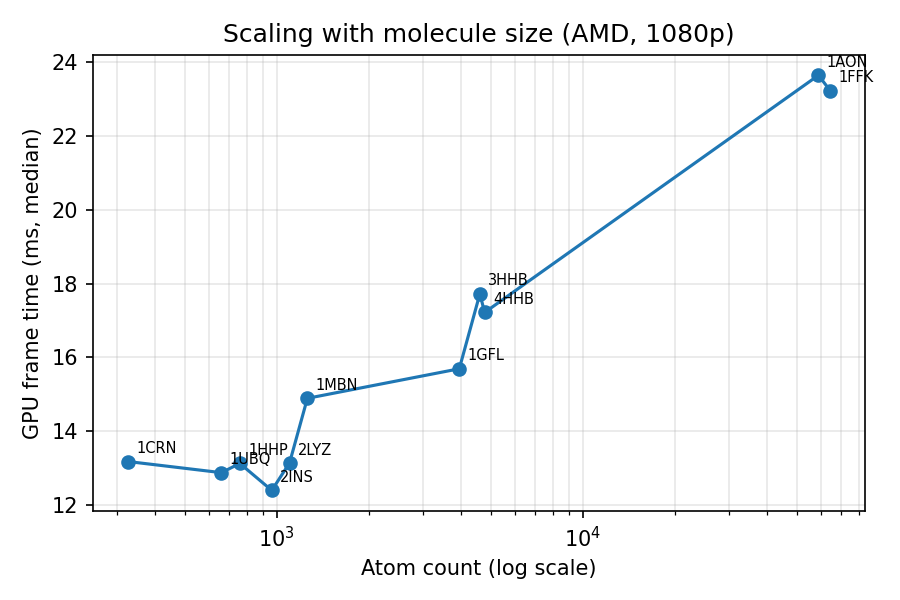
\includegraphics[width=0.75\textwidth]{scaling_amd.png}
    \caption{GPU frame time vs.\ atom count (AMD, 1080p, log scale). The plateau below 1000 atoms confirms the pipeline is fill-bound for small proteins. Even at 60k atoms the frame time stays below 25~ms.}
    \label{fig:scaling_amd}
\end{figure}

\begin{figure}[H]
    \centering
    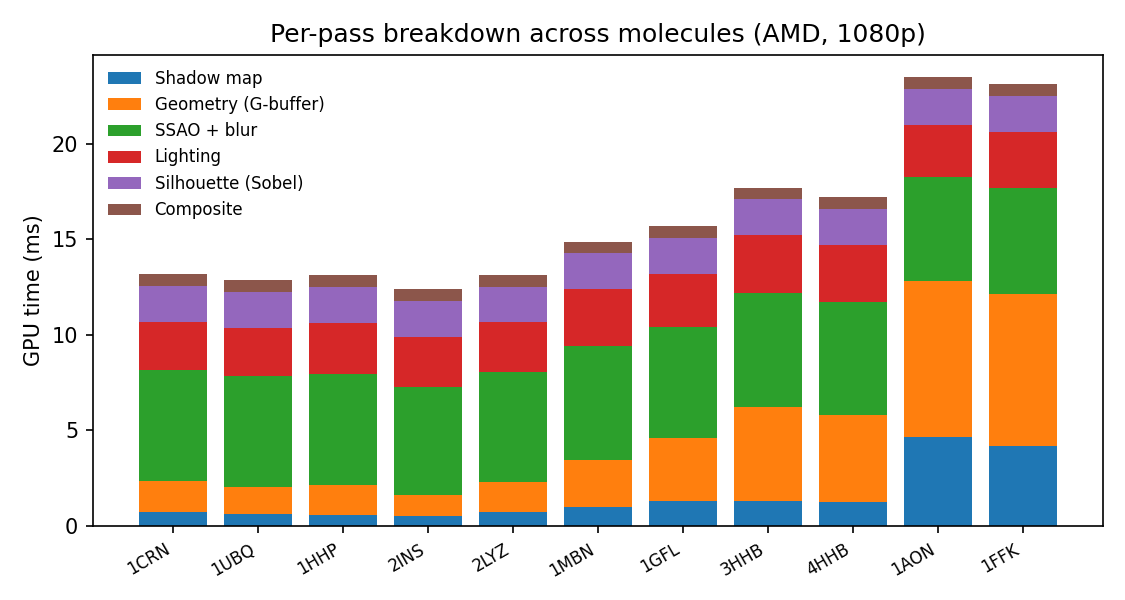
\includegraphics[width=0.95\textwidth]{pass_breakdown_amd.png}
    \caption{Per-pass breakdown across all 11 molecules (AMD, 1080p). SSAO and lighting are roughly constant because they depend on screen area; geometry and shadow grow with atom count. The same pass ordering holds on the M3; the relative proportions are nearly identical, with SSAO at $\approx$41\% of the pass total.}
    \label{fig:pass_breakdown_amd}
\end{figure}

The frame time plateaus around 13~ms up to ~1000 atoms (fill-bound by SSAO and lighting), then rises gradually. At 60k atoms it reaches 24~ms (43~FPS), still fully interactive. Figure~\ref{fig:pass_breakdown_amd} shows the per-pass cost breakdown across all molecules. Both machines follow the same shape; Figure~\ref{fig:compare_scaling} overlays them.

\begin{figure}[H]
    \centering
    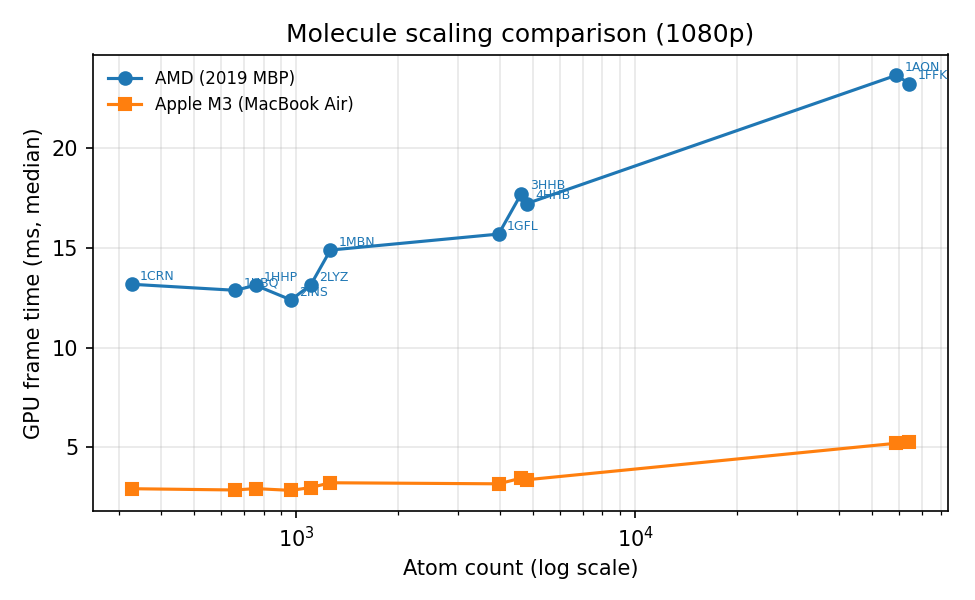
\includegraphics[width=0.85\textwidth]{compare_scaling.png}
    \caption{GPU frame time vs.\ atom count for both machines (1080p). The M3 curve sits consistently lower, reflecting the TBDR bandwidth advantage.}
    \label{fig:compare_scaling}
\end{figure}

\subsection{Resolution scaling}

Table~\ref{tab:compare_resolution} shows the total GPU frame time for 1HHP at three resolutions.

\begin{table}[H]
    \centering
    \small
    \begin{tabular}{lrrrr}
        \toprule
        Resolution & FB pixels & AMD (ms) & M3 (ms) & Speedup \\
        \midrule
        720p & 1280$\times$720 & 6.78 & 1.12 & 6.0$\times$ \\
        1080p & 1920$\times$1080 & 13.13 & 2.94 & 4.5$\times$ \\
        native & 2880$\times$1800 & 31.05 & 6.77 & 4.6$\times$ \\
        \bottomrule
    \end{tabular}
    \caption{Resolution scaling comparison, molecule 1HHP HIV-PR. GPU total frame time (ms, median over 300 frames).}
    \label{tab:compare_resolution}
\end{table}


Fill-bound passes (SSAO, lighting, silhouette) grow almost linearly with pixel count; the shadow pass, which renders to its own fixed-size $2048\times2048$ map, stays constant across resolutions. The AMD machine drops to 32~FPS at the native panel resolution; the M3 stays at 148~FPS.

\subsection{Feature ablation}

Table~\ref{tab:compare_ablation} isolates the cost of each optional feature at 1080p.

\begin{table}[H]
    \centering
    \small
    \begin{tabular}{lrrrr}
        \toprule
        Configuration & AMD (ms) & AMD FPS & M3 (ms) & M3 FPS \\
        \midrule
        Full pipeline & 13.13 & 76 & 2.94 & 340 \\
        No shadows & 10.92 & 92 & 2.59 & 386 \\
        No SSAO & 7.33 & 136 & 2.19 & 456 \\
        No outlines & 12.10 & 83 & 2.79 & 359 \\
        Bare & 4.07 & 246 & 1.37 & 729 \\
        \bottomrule
    \end{tabular}
    \caption{Feature ablation on both machines at 1080p, molecule 1HHP HIV-PR.}
    \label{tab:compare_ablation}
\end{table}


SSAO is the most expensive optional feature on both machines. Disabling it adds roughly 5.8~ms on AMD and 0.75~ms on M3, pushing the AMD frame rate from 76 to 136~FPS. The \emph{bare} configuration (geometry + lighting + composite only) runs at 245~FPS (AMD) and 729~FPS (M3), setting the cost floor of the pipeline.
\needspace{10\baselineskip} % 10
\subsection{CPU load times}

Figure~\ref{fig:load_amd} and Table~\ref{tab:load_amd} show PDB parse and bond-detection times (five measured runs, median).

\begin{table}[H]
    \centering
    \small
    \begin{tabular}{lrrrrrr}
        \toprule
        Molecule & Atoms & Bonds & Parse (ms) & Bond detect (ms) & Predicted $O(N^2)$ (ms) & Total (ms) \\
        \midrule
        1CRN & 327 & 337 & 0.44 & 0.51 & 0.51 & 0.95 \\
        1UBQ & 660 & 608 & 0.76 & 2.00 & 2.08 & 2.76 \\
        1HHP & 758 & 771 & 0.80 & 2.39 & 2.74 & 3.19 \\
        2INS & 964 & 810 & 1.10 & 3.56 & 4.43 & 4.66 \\
        2LYZ & 1102 & 1037 & 1.08 & 5.06 & 5.79 & 6.14 \\
        1MBN & 1260 & 1298 & 1.33 & 7.28 & 7.57 & 8.62 \\
        1GFL & 3950 & 3738 & 3.04 & 62.10 & 74.43 & 65.13 \\
        3HHB & 4612 & 4704 & 3.55 & 87.46 & 101.46 & 91.01 \\
        4HHB & 4779 & 4633 & 3.96 & 94.39 & 108.94 & 98.34 \\
        1AON & 58870 & 59307 & 37.97 & 13416.80 & 16531.59 & 13454.70 \\
        1FFK & 64281 & 67866 & 42.76 & 17757.00 & 19710.24 & 17799.70 \\
        \bottomrule
    \end{tabular}
    \caption{PDB parse and bond detection times on the AMD machine (median of 5 runs). The predicted $O(N^2)$ column scales the bond detection time of the smallest molecule (1CRN) by $(N/N_{1CRN})^2$. The close match confirms the quadratic growth of the pairwise distance check.}
    \label{tab:load_amd}
\end{table}


\begin{figure}[H]
    \centering
    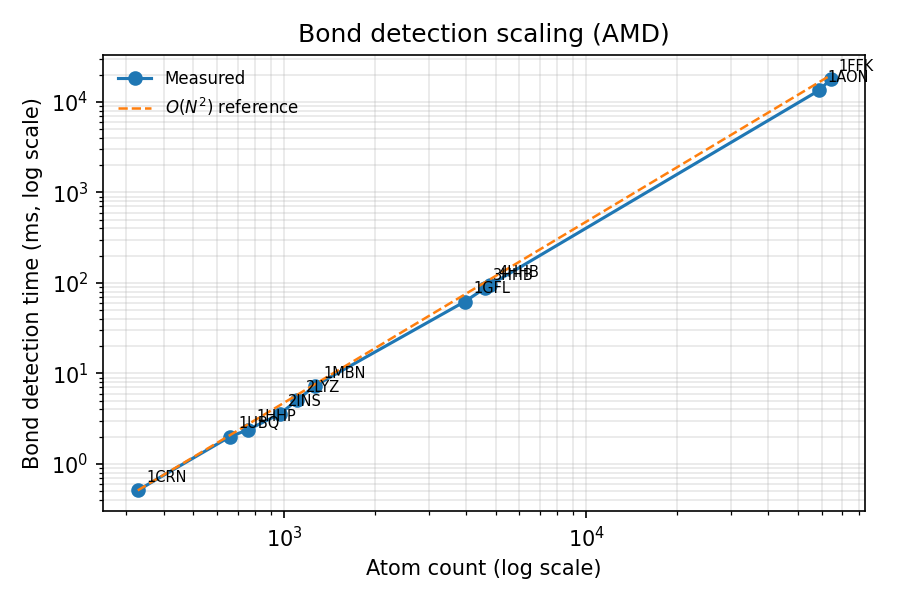
\includegraphics[width=0.80\textwidth]{load_amd.png}
    \caption{Bond detection time vs.\ atom count (AMD, log-log). Measured values (blue) follow the $O(N^2)$ reference line (dashed) closely, confirming the pairwise distance check is genuinely quadratic.}
    \label{fig:load_amd}
\end{figure}

Parsing scales linearly and stays below 45~ms. Bond detection is the bottleneck: for 1AON (58\,870 atoms) and 1FFK (64\,281 atoms) it takes 13.4 and 17.8~seconds respectively, matching the predicted $O(N^2)$ value to within 20\%. For all molecules under 5000 atoms the total load time is below 100~ms. A spatial index (uniform grid or k-d tree) would reduce this to $O(N \log N)$.
\needspace{10\baselineskip} % 10
\subsection{Discussion}

Three conclusions follow from the data. First, geometry submission is cheap: instanced rendering keeps the geometry pass well below a few milliseconds even at 60k atoms. Second, \textbf{SSAO} is the primary GPU bottleneck, accounting for 40--50\% of the frame budget at 1080p; a half-resolution SSAO target with bilateral upsampling would have the largest impact on performance. Finally, the pipeline scales predictably: \textbf{fill-bound passes} grow linearly with framebuffer area, the \textbf{shadow pass} is resolution-independent, and no super-linear degradation was observed.

When comparing these findings with the reference paper~\cite{sigg2006} in relative terms, Sigg et al.\ report that the silhouette pass occupies approximately 8\% of their frame budget, while our implementation accounts for roughly 14--17\%. This variance is structurally plausible given that our Sobel filter executes at full screen resolution, whereas theirs used a dedicated edge-detection pass at reduced resolution.
\clearpage
% =========================================================================
\section{Conclusion}
% =========================================================================

This project successfully implements the GPU ray-casting method of Sigg et al.~\cite{sigg2006} within a modern deferred shading pipeline. Sphere and cylinder impostors produce pixel-perfect silhouettes and surface normals at any zoom level, with no tessellation artefacts. Benchmarks on two machines confirm that the full pipeline is interactive across the entire test set: on the AMD MBP 2019 it delivers 76~FPS at 1080p for a mid-size protein (758 atoms) and stays above 42~FPS even for a 64k-atom ribosome; on the Apple~M3 the same pipeline reaches 340~FPS and 140~FPS respectively, a $4.5\times$ advantage attributable to the tile-based GPU architecture.

The most significant technical insight encountered during development was the numerical instability of the paper's parameter-space ray transformation under perspective at large zoom-out distances. Solving the intersection directly in eye space avoids the ill-conditioned matrix inversion and is mathematically equivalent for spheres. A second key insight was the importance of the tight NDC bounding box (eq.~\ref{eq:spherenndc}): without it, atom silhouettes are clipped at close range because the eye-space billboard expansion underestimates the true screen extent of the sphere.

\subsection{Limitations}

Several aspects of the current implementation present known technical limitations. First, the \textbf{bond detection complexity} relies on a pairwise distance check, resulting in an $O(N^2)$ performance cost relative to the number of atoms. While this approach remains acceptable for proteins containing a few thousand atoms, it introduces a noticeable computational delay when processing massive structures such as GroEL ($\approx 58\,000$ atoms) or the ribosome ($\approx 100\,000$ atoms). Integrating a spatial acceleration structure, such as a \textbf{uniform grid} or a \textbf{k-d tree}, would effectively reduce this complexity to $O(N \log N)$. Finally, the current shading architecture is restricted to a \textbf{single directional light source}; consequently, advanced illumination methods such as \textit{point lights}, \textit{area lights}, and \textit{image-based lighting} are not currently implemented.

\subsection{Future Work}

\begin{itemize}
    \item \textbf{Spatial acceleration for bond detection.} Replace the $O(N^2)$ pairwise 
    distance check with a uniform grid or k-d tree to make large-molecule loading 
    interactive ($O(N \log N)$).
    \item \textbf{Representation toggle.} A space-fill mode (van der Waals spheres only, 
    no cylinders) requires only disabling the cylinder draw call and adjusting atom radii.
    \item \textbf{Per-atom selection and highlighting.} Atom picking via framebuffer 
    object-ID rendering; highlight selected atoms with an outline or colour change.
    \item \textbf{Extended colouring schemes.} Currently only CPK colouring is supported; 
    per-chain, per-residue-type, or B-factor heat-map colouring are natural additions.
    \item \textbf{Runtime PDB loading.} The molecule list is currently hardcoded to 11 
    entries; a file-picker would make the viewer a general-purpose tool.
\end{itemize} 
\clearpage
% =========================================================================
\begin{thebibliography}{9}

\bibitem{sigg2006}
Sigg, C., Weyrich, T., Botsch, M., \& Gross, M. (2006).
\textit{GPU-Based Ray-Casting of Quadratic Surfaces.}
Eurographics Symposium on Point-Based Graphics.
\url{http://reality.cs.ucl.ac.uk/projects/quadrics/pbg06.pdf}

\bibitem{bondi1964}
Bondi, A. (1964).
van der Waals Volumes and Radii.
\textit{Journal of Physical Chemistry}, 68(3), 441--451.
\url{https://doi.org/10.1021/j100785a001}

\bibitem{alvarez2008}
Alvarez, S. (2008).
Are the radii of atoms constant in chemical combinations?
\textit{Dalton Transactions}, 2832--2838.
\url{https://doi.org/10.1039/b801115j}

\bibitem{cpk}
Corey, R. B., \& Pauling, L. (1953).
Molecular models of amino acids, peptides, and proteins.
\textit{Review of Scientific Instruments}, 24(8), 621--627.

\bibitem{pdb}
Berman, H. M., et al. (2000).
The Protein Data Bank.
\textit{Nucleic Acids Research}, 28(1), 235--242.
\url{https://doi.org/10.1093/nar/28.1.235}

\end{thebibliography}

\end{document}
